\documentclass{beamer}
\usepackage[utf8]{inputenc}
\usepackage{graphicx, epsfig}
\usepackage{amsmath,mathrsfs,amsfonts,amssymb}
%\usepackage{subfig}
\usepackage{floatflt}
\usepackage{epic,ecltree}
\usepackage{mathtext}
\usepackage{fancybox}
\usepackage{fancyhdr}
\usepackage{multirow}
\usepackage{enumerate}
\usepackage{epstopdf}
\usepackage{multicol}
\usepackage{algorithm}
\usepackage[noend]{algorithmic}
\def\algorithmicrequire{\textbf{Input:}}
\def\algorithmicensure{\textbf{Output:}}
\usetheme{default}%{Singapore}%{Warsaw}%{Warsaw}%{Darmstadt}
\usecolortheme{default}
\setbeamerfont{title}{size=\Huge}
\setbeamertemplate{footline}[page number]{}
\setbeamerfont{title}{size=\Huge}
\beamertemplatenavigationsymbolsempty

% latin bold lower
\newcommand{\ba}{\mathbf{a}} 
\newcommand{\bc}{\mathbf{c}} 
\newcommand{\be}{\mathbf{e}} 
\newcommand{\bh}{\mathbf{h}} 
\newcommand{\bp}{\mathbf{p}} 
\newcommand{\bt}{\mathbf{t}} 
\newcommand{\bu}{\mathbf{u}} 
\newcommand{\bv}{\mathbf{v}} 
\newcommand{\bw}{\mathbf{w}} 
\newcommand{\bx}{\mathbf{x}} 
\newcommand{\by}{\mathbf{y}} 
\newcommand{\bz}{\mathbf{z}} 

% latin bold upper
\newcommand{\bA}{\mathbf{A}} 
\newcommand{\bC}{\mathbf{C}} 
\newcommand{\bI}{\mathbf{I}} 
\newcommand{\bM}{\mathbf{M}} 
\newcommand{\bT}{\mathbf{T}} 
\newcommand{\bU}{\mathbf{U}} 
\newcommand{\bW}{\mathbf{W}} 
\newcommand{\bX}{\mathbf{X}} 
\newcommand{\bY}{\mathbf{Y}} 
\newcommand{\bZ}{\mathbf{Z}} 

% latin cal upper
\newcommand{\cL}{\mathcal{L}} 
\newcommand{\cN}{\mathcal{N}} 
\newcommand{\cS}{\mathcal{S}} 
\newcommand{\cT}{\mathcal{T}} 
\newcommand{\cW}{\mathcal{W}} 
\newcommand{\cX}{\mathcal{X}} 
\newcommand{\cZ}{\mathcal{Z}} 

% latin cal upper
\newcommand{\bbE}{\mathbb{E}} 
\newcommand{\bbP}{\mathbb{P}} 
\newcommand{\bbR}{\mathbb{R}} 

% greek bold lower
\newcommand{\bepsilon}{\boldsymbol{\epsilon}} 
\newcommand{\btheta}{\boldsymbol{\theta}} 
\newcommand{\blambda}{\boldsymbol{\lambda}} 
\newcommand{\bmu}{\boldsymbol{\mu}} 
\newcommand{\bsigma}{\boldsymbol{\sigma}} 
\newcommand{\bphi}{\boldsymbol{\phi}} 

% greek bold upper
\newcommand{\bSigma}{\boldsymbol{\Sigma}} 

\DeclareMathOperator*{\argmin}{arg\,min}
\DeclareMathOperator*{\argmax}{arg\,max}

\newcommand{\createdgmtitle}[1]{\title[\hbox to 56mm{Deep Generative Models  \hfill\insertframenumber\,/\,\inserttotalframenumber}]
	{\vspace{1cm} \\ Deep Generative Models \\ Lecture #1 \\ \vspace{-0.5cm}}
	\author{Roman Isachenko \\ \vspace{-0.5cm}}
	\institute{
\includegraphics[width=3cm]{../utils/ozonmasterslogo}
	\\Ozon Masters
	}
	\date{Spring, 2021}
}

\newcommand\myfootnote[1]{%
  \tikz[remember picture,overlay]
  \draw (current page.south west) +(1in + \oddsidemargin,0.5em)
  node[anchor=south west,inner sep=0pt]{\parbox{\textwidth}{%
      \rlap{\rule{10em}{0.4pt}}\raggedright\scriptsize#1}};}

\newcommand\myfootnotewithlink[2]{%
  \tikz[remember picture,overlay]
  \draw (current page.south west) +(1in + \oddsidemargin,0.5em)
  node[anchor=south west,inner sep=0pt]{\parbox{\textwidth}{%
      \rlap{\rule{10em}{0.4pt}}\raggedright\scriptsize\href{#1}{\textit{#2}}}};}
\createdgmtitle{1}
%--------------------------------------------------------------------------------
\begin{document}
%--------------------------------------------------------------------------------
\begin{frame}
%\thispagestyle{empty}
\titlepage
\end{frame}
%--------------------------------------------------------------------------------
\section{Logistics}
%=======
\begin{frame}{Logistics}
    \begin{itemize}
        \item homeworks: 30 points
        \begin{itemize}
            \item hw1: autoregressive models
            \item hw2: latent variable models
            \item hw3: flow models
            \item hw4: adversarial models
        \end{itemize}
        \item exam: 30 points
        \item final project: 40 points
    \end{itemize}
    Last year course page: \href{http://bit.ly/IS_B2}{link} \\
    Admission: \href{https://docs.google.com/spreadsheets/d/1FpTneCfkYNIG1FMxG7ALTwMCGDngkqc_OJC6SDqeG0Q/edit?usp=sharing}{link}
\end{frame}
%--------------------------------------------------------------------------------
\section{Intro}
%=======
\begin{frame}{Generative models zoo}
    \begin{figure}
        \centering
        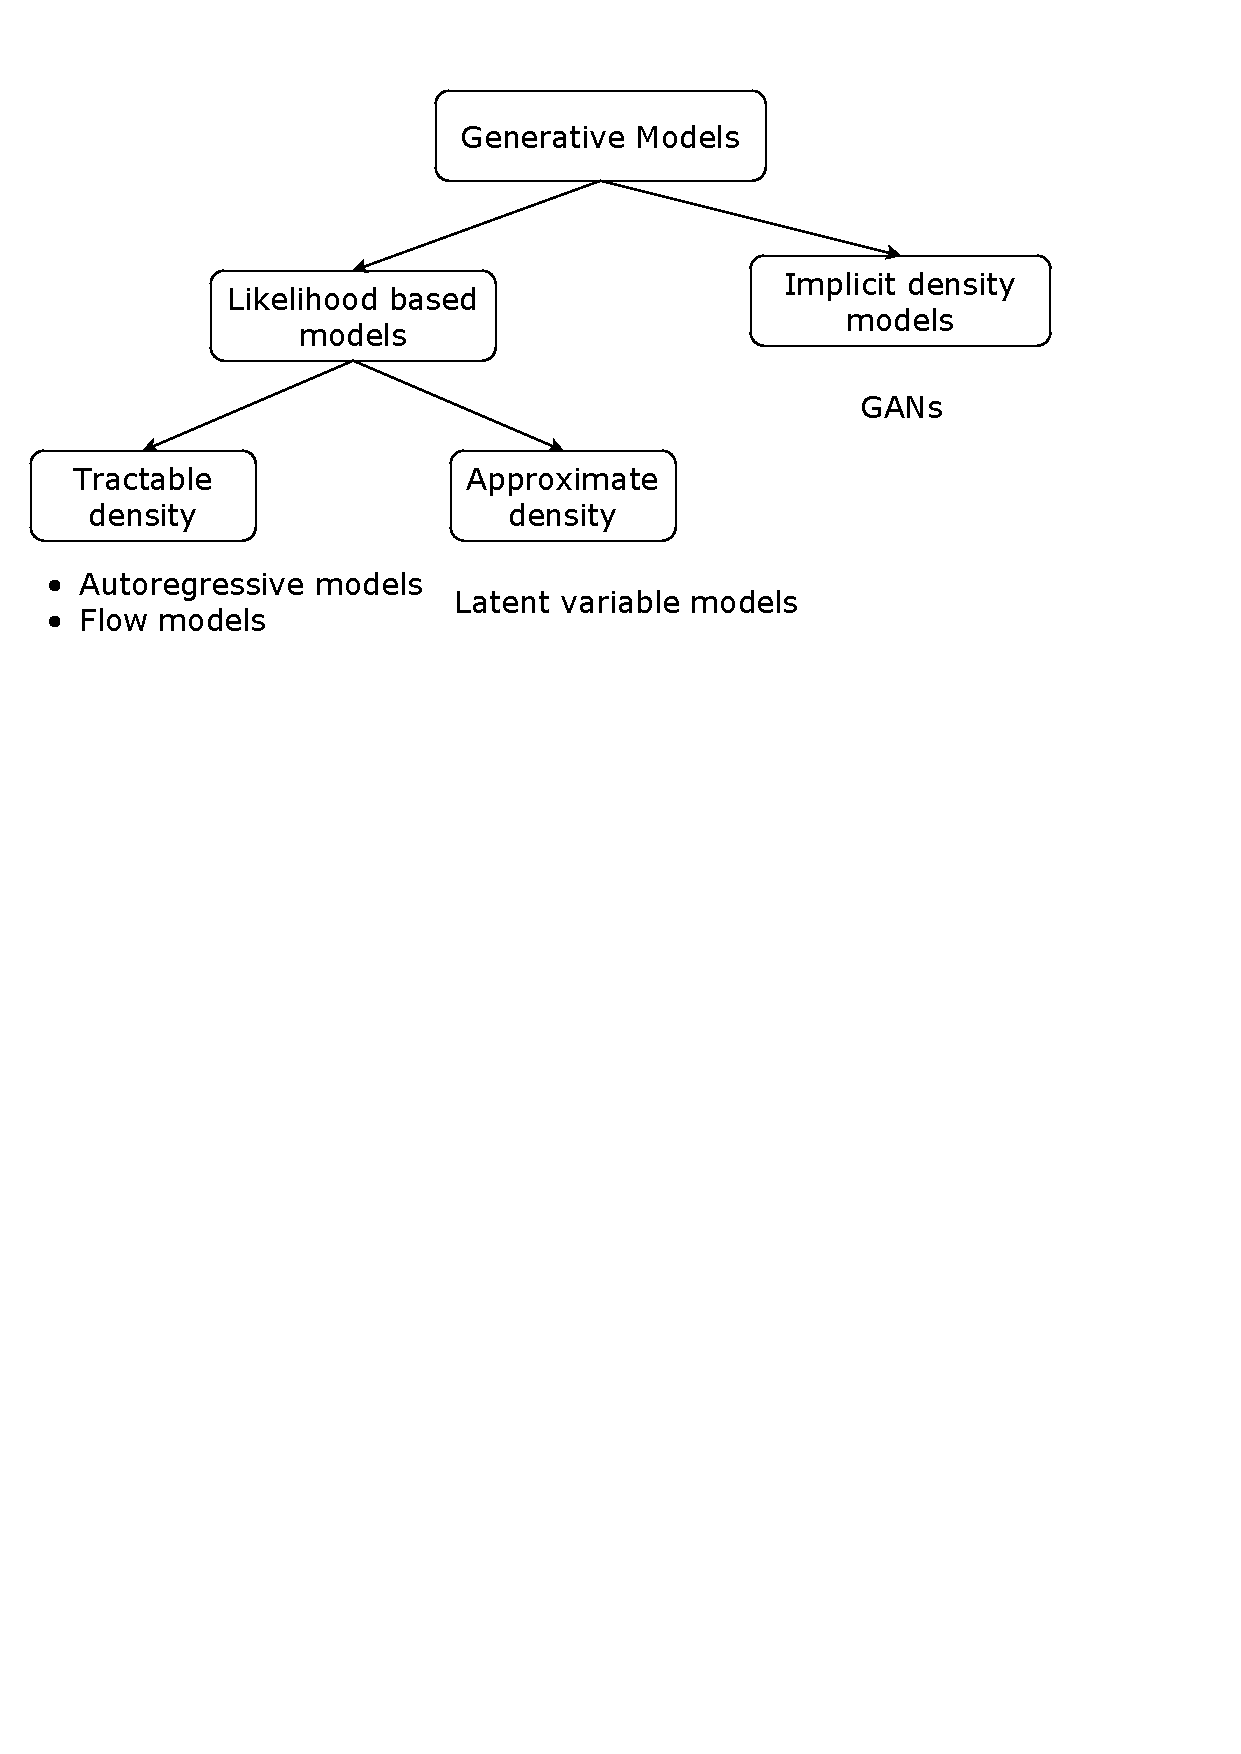
\includegraphics[width=1.0\linewidth]{figs/generative_models_zoo.pdf}
        \label{fig:generative_models_zoo}
    \end{figure}
\end{frame}
%=======
\begin{frame}{Applications}
	\begin{figure}
		\centering
		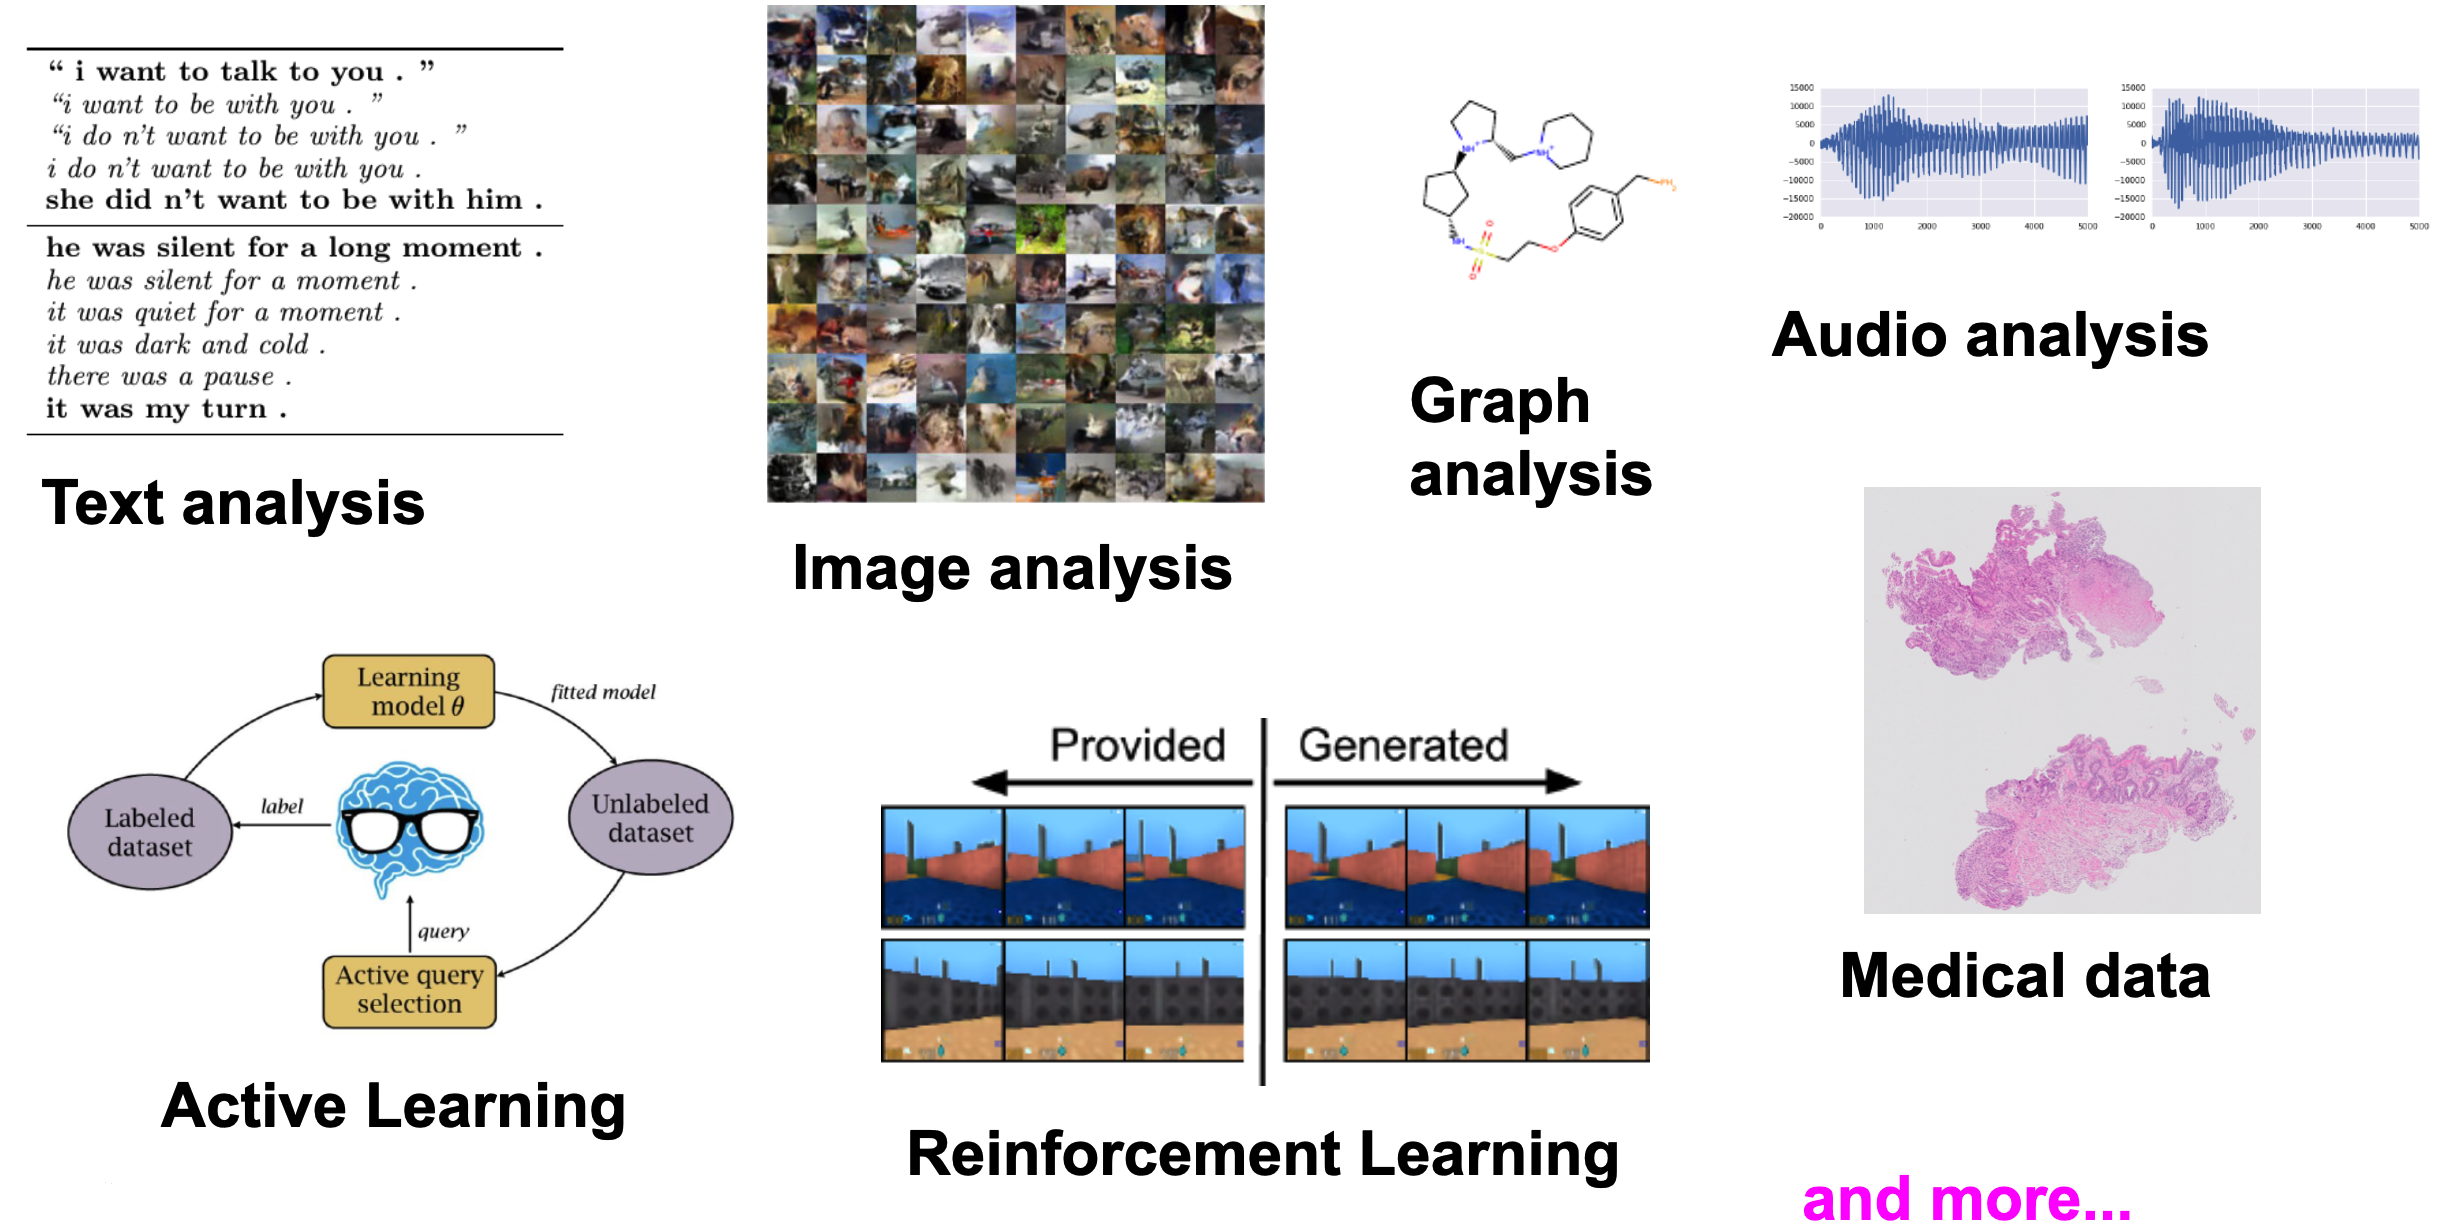
\includegraphics[width=\linewidth]{figs/applications}
	\end{figure}
\end{frame}
%=======
\begin{frame}{Applications: Image generation (VAE)}
    \begin{figure}
        \centering
        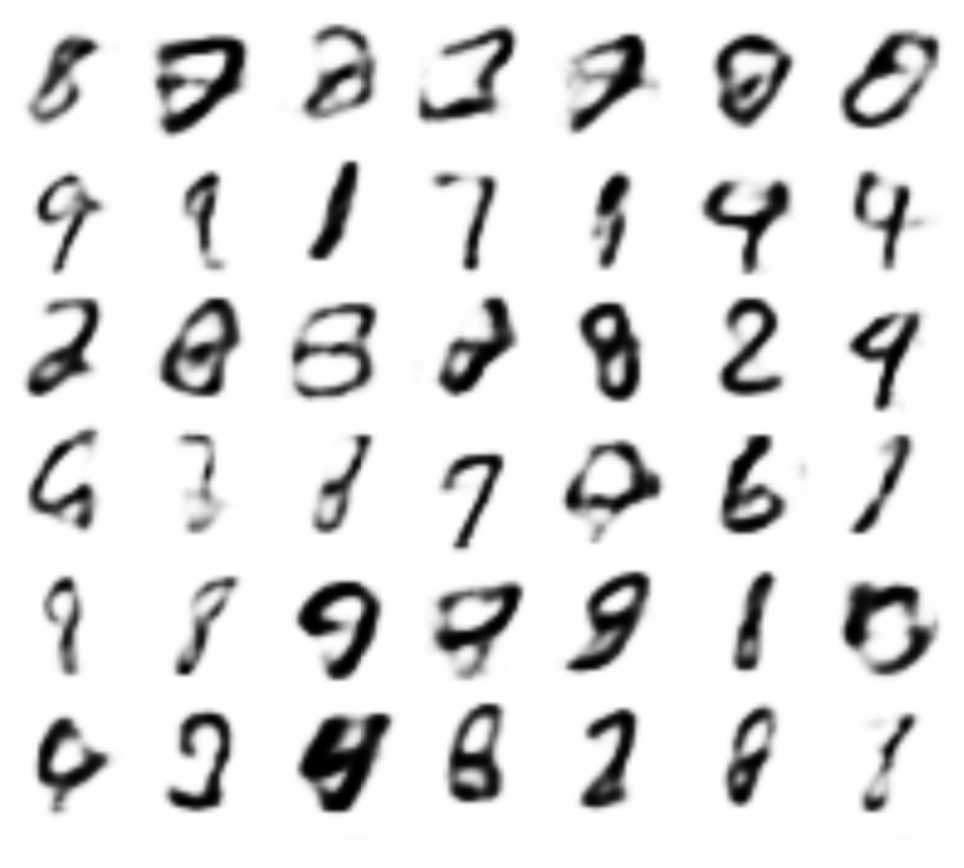
\includegraphics[width=0.8\linewidth]{figs/vae.png}
    \end{figure}
\myfootnotewithlink{https://arxiv.org/abs/1312.6114}{Kingma D. P., Welling M. Auto-encoding variational bayes, 2013}
\end{frame}
%=======
\begin{frame}{Applications: Image generation (DCGAN)}
    \begin{figure}
        \centering
        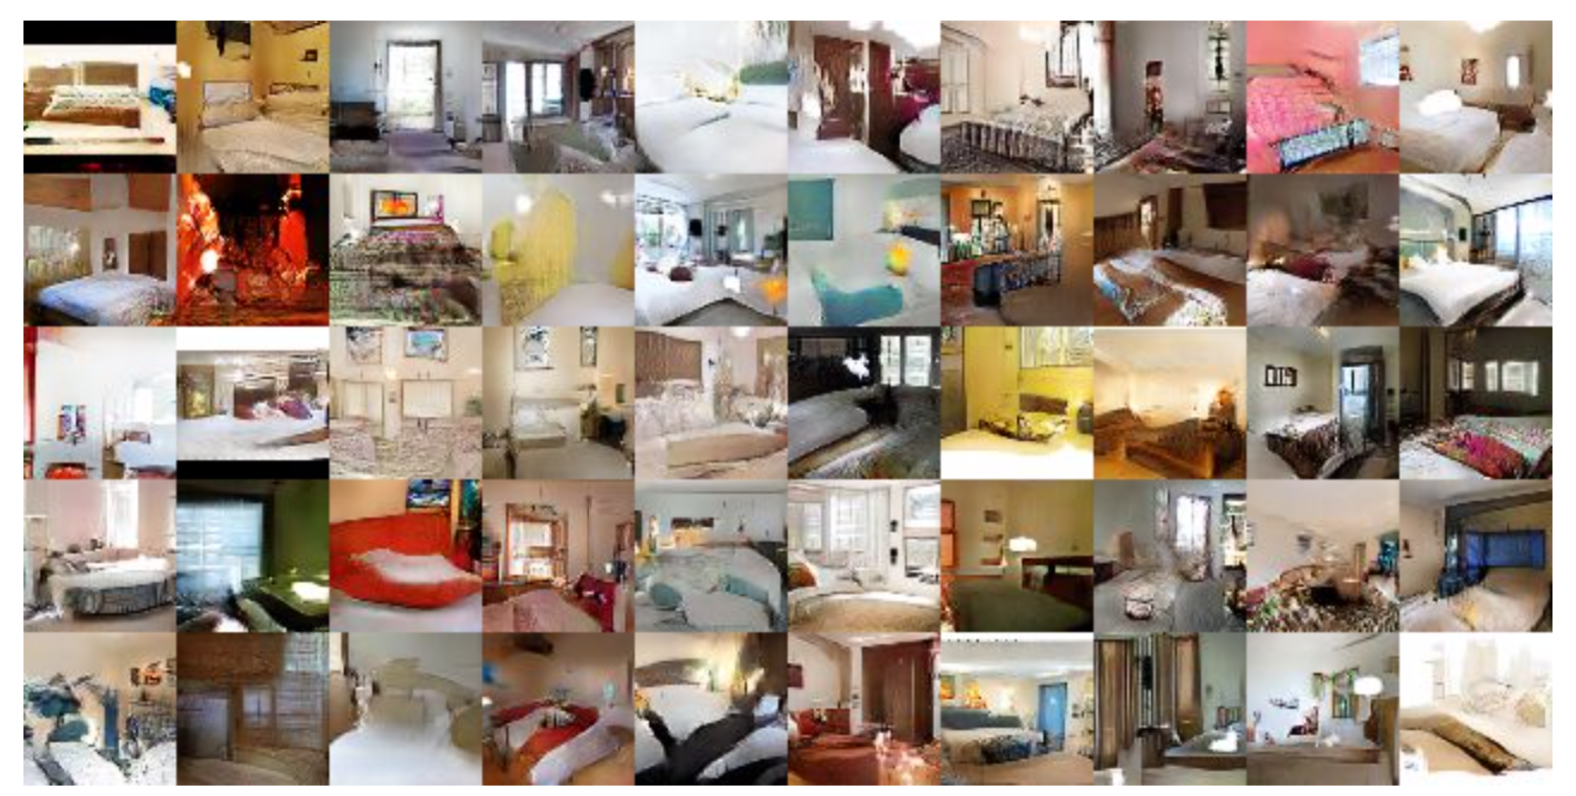
\includegraphics[width=1.0\linewidth]{figs/dcgan.png}
    \end{figure}
\myfootnotewithlink{https://arxiv.org/abs/1511.06434}{Radford A., Metz L., Chintala S. Unsupervised representation learning with deep convolutional generative adversarial networks, 2015}
\end{frame}
%=======
\begin{frame}{Applications: SuperResolution (SRGAN)}
    \begin{figure}
        \centering
        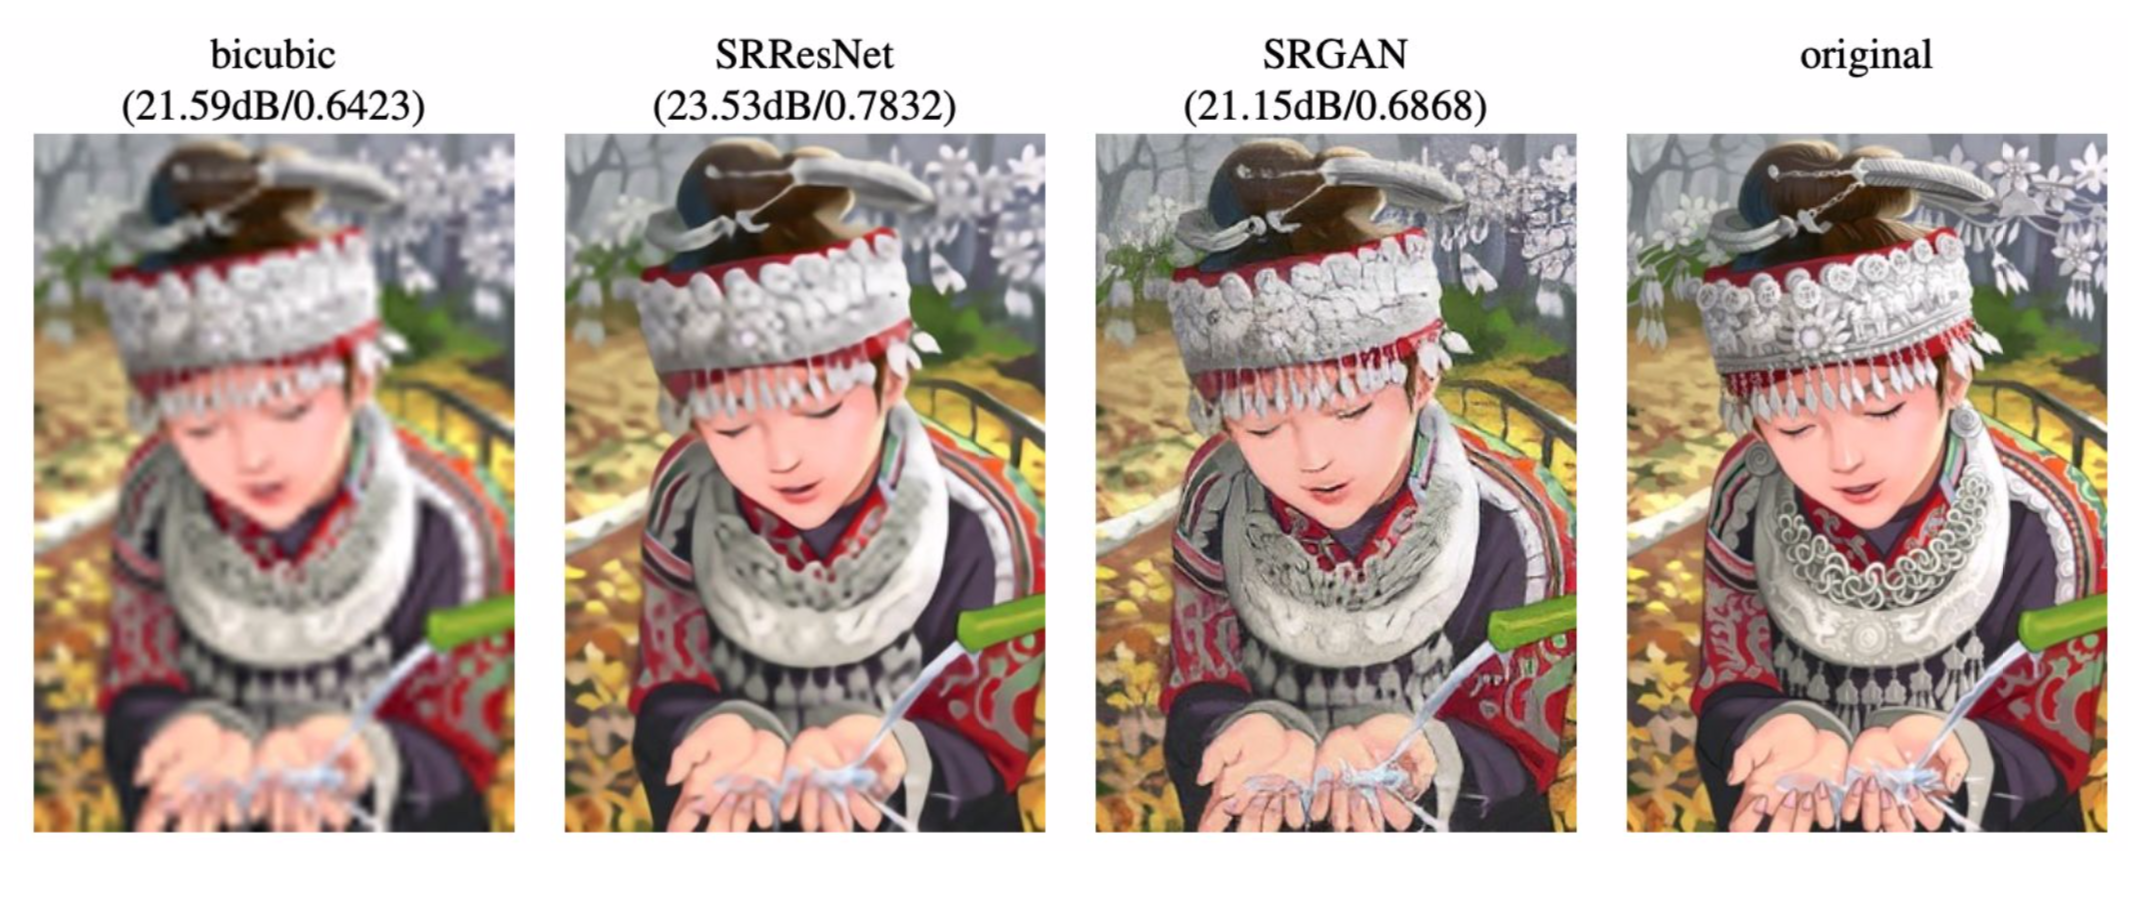
\includegraphics[width=1.0\linewidth]{figs/srgan.png}
        \label{fig:srgan}
    \end{figure}
\myfootnotewithlink{https://arxiv.org/abs/1609.04802}{Ledig C. et al. Photo-realistic single image super-resolution using a generative adversarial network, 2016}
\end{frame}
%=======
\begin{frame}{Applications: Face generation (StyleGAN)}
	\begin{figure}
		\centering
		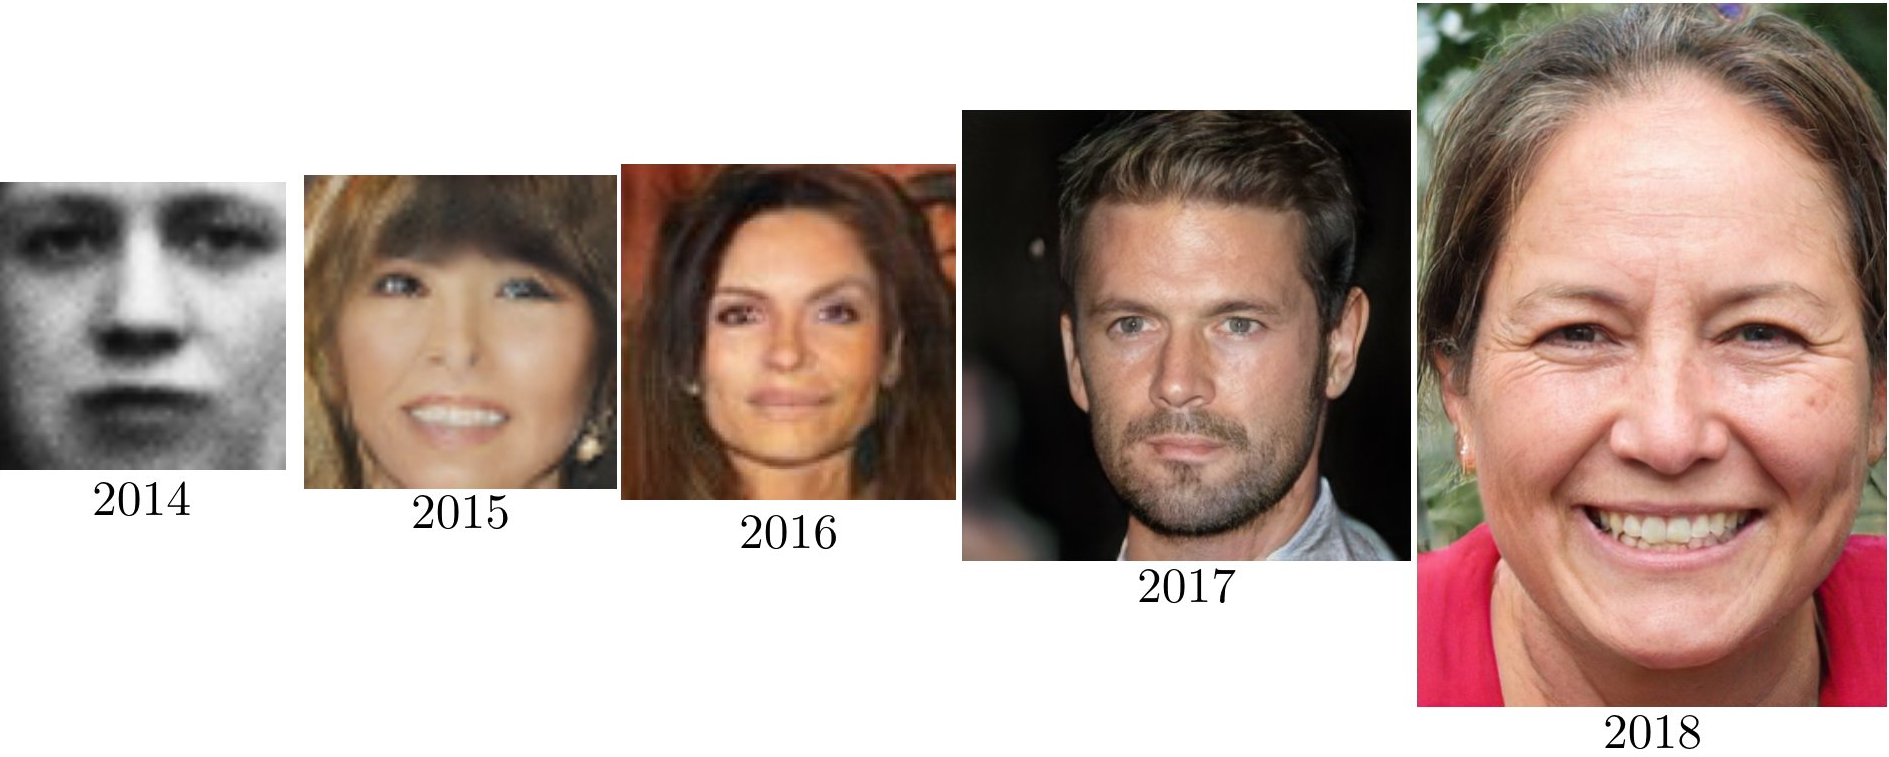
\includegraphics[width=0.85\linewidth]{figs/gan_evolution}
	\end{figure}
	\vspace{-0.2cm}
	\begin{figure}
		\centering
		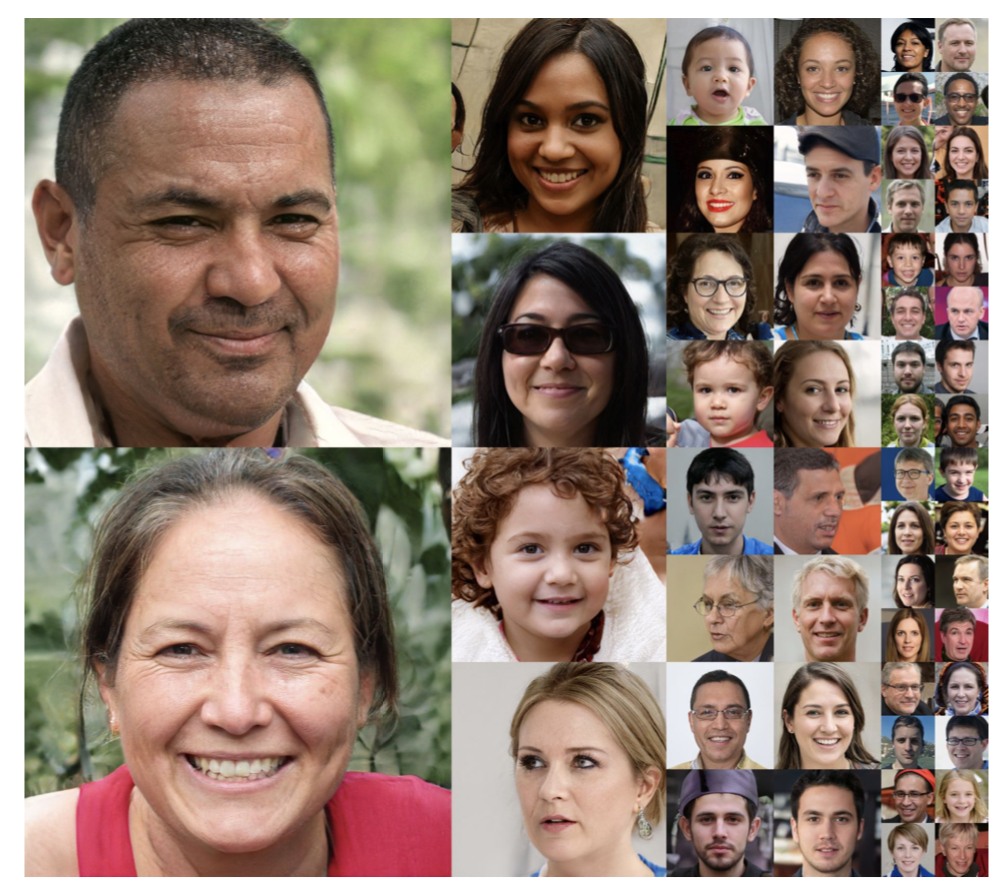
\includegraphics[width=0.75\linewidth]{figs/stylegan}
	\end{figure}
	\myfootnotewithlink{https://arxiv.org/abs/1812.04948}{Karras T., Laine S., Aila T. A style-based generator architecture for generative adversarial networks, 2018}
\end{frame}
%=======
\begin{frame}{Applications: Face generation (VQ-VAE-2)}
    \begin{figure}
        \centering
        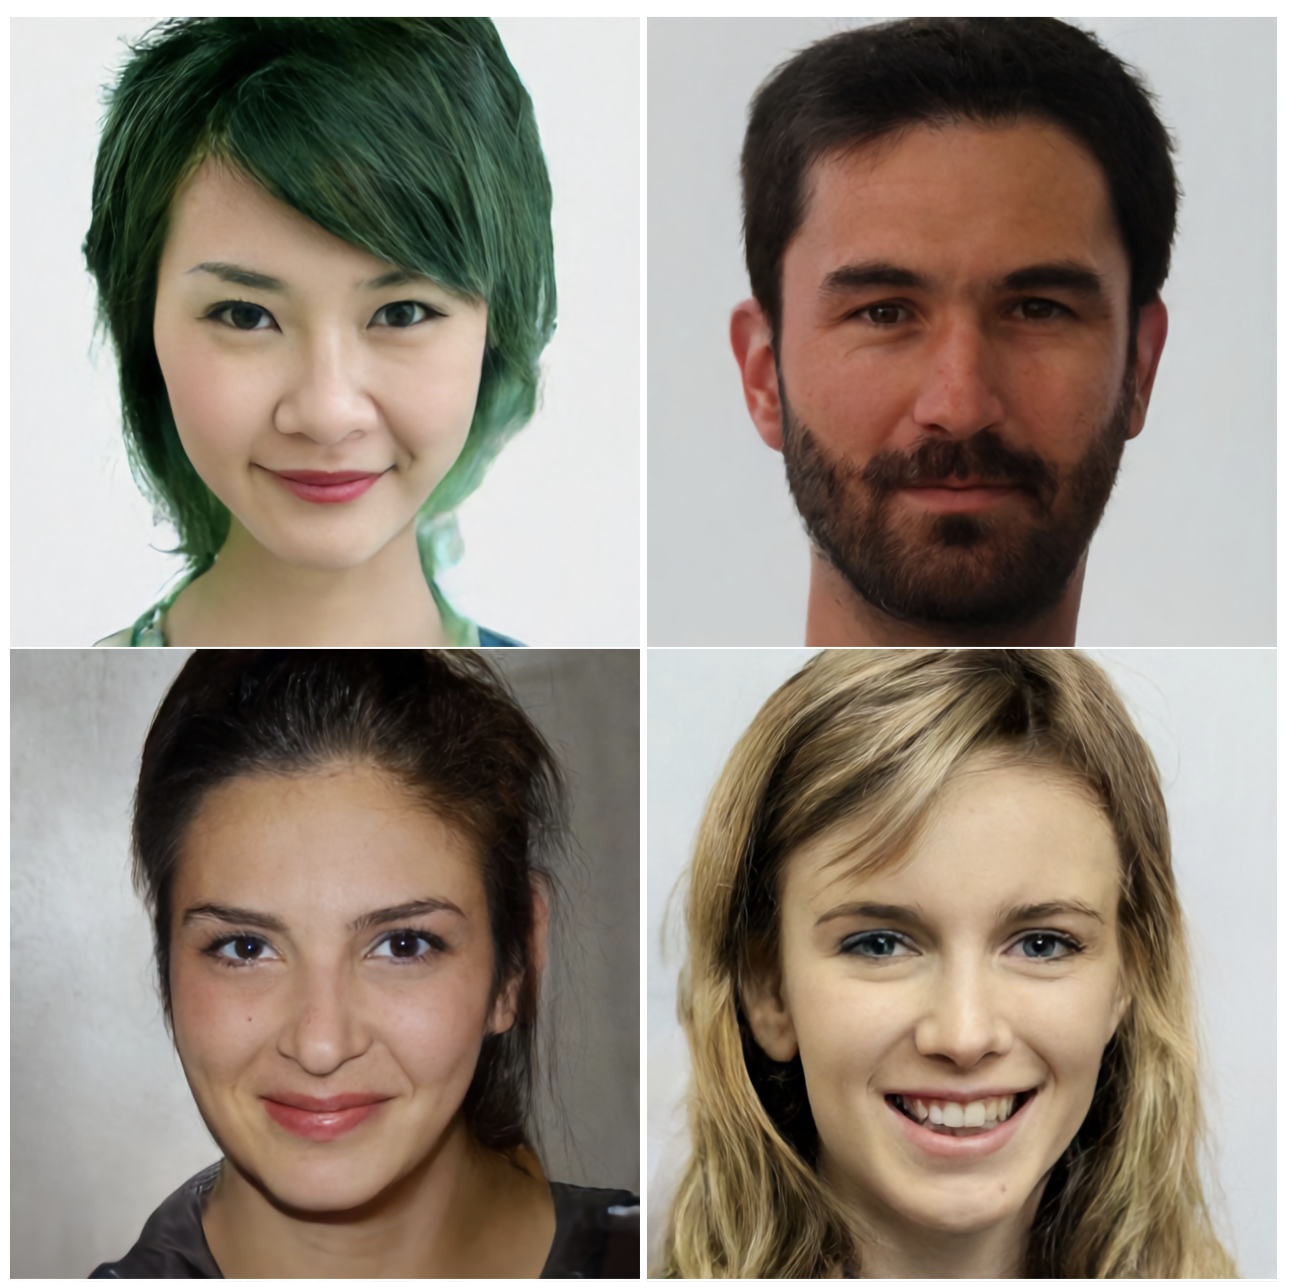
\includegraphics[width=0.7\linewidth]{figs/vq_vae.png}
    \end{figure}
\myfootnotewithlink{https://arxiv.org/abs/1906.00446}{Razavi A., Oord A., Vinyals O. Generating Diverse High-Fidelity Images with VQ-VAE-2, 2019}
\end{frame}
%=======
\begin{frame}{Applications: Language modelling}
	\begin{figure}
		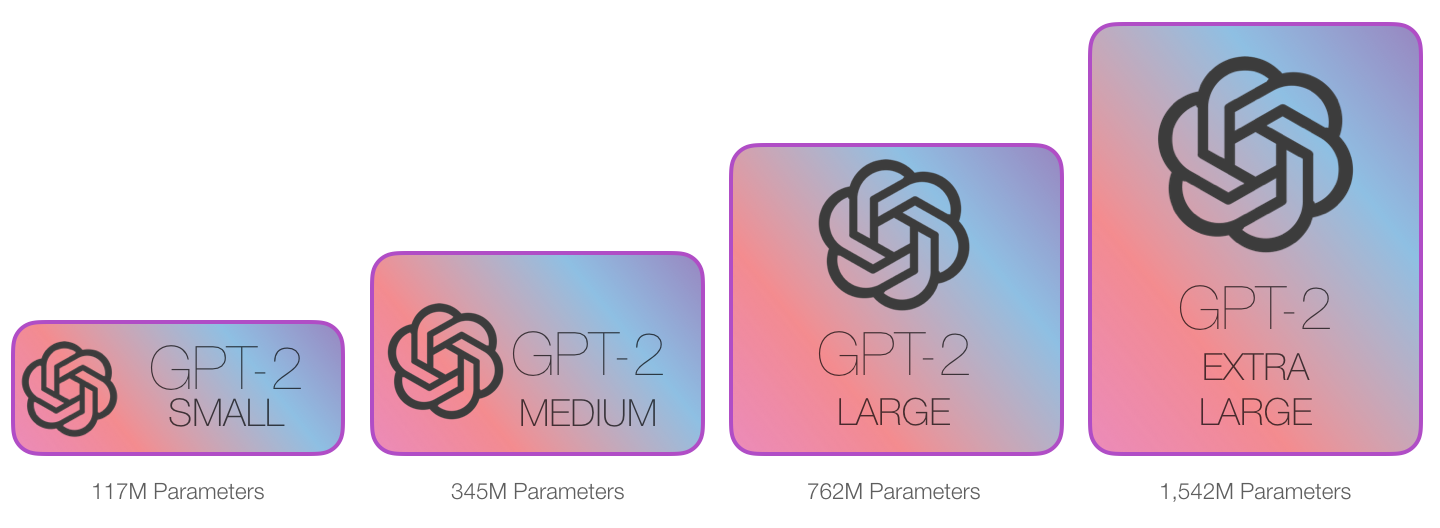
\includegraphics[width=0.65\linewidth]{figs/gpt2-sizes}
	\end{figure}
	\vspace{-0.2cm}
	\begin{figure}
		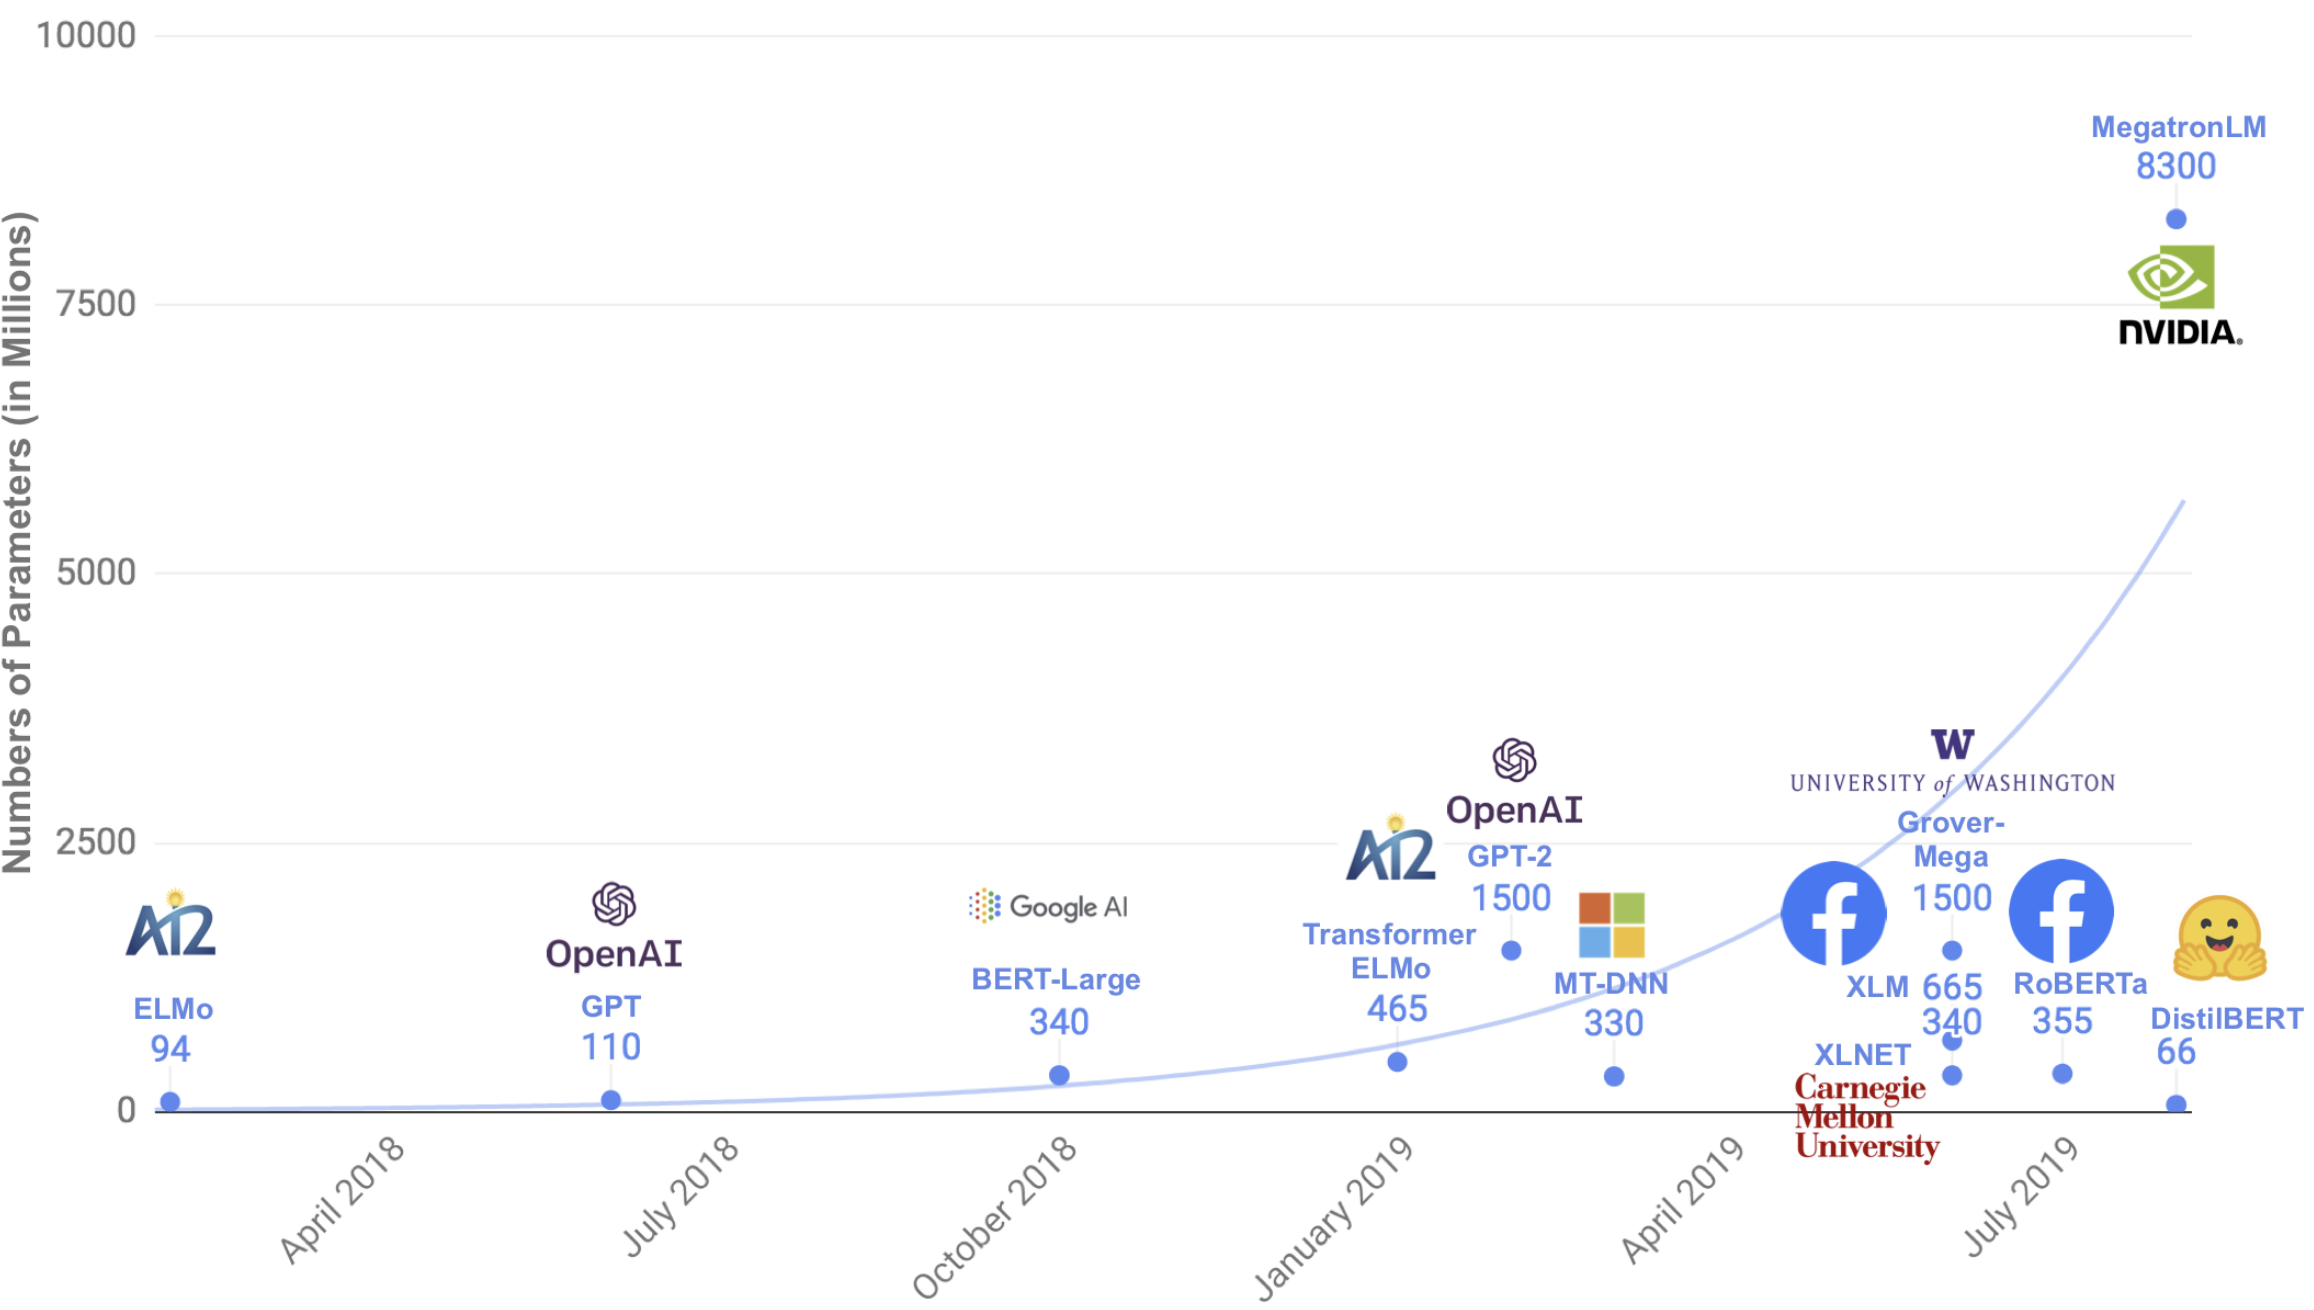
\includegraphics[width=0.7\linewidth]{figs/nlp_models}
	\end{figure}
\myfootnote{\href{http://jalammar.github.io/illustrated-gpt2}{image credit: http://jalammar.github.io/illustrated-gpt2} \\
\href{https://arxiv.org/abs/1910.01108}{Sanh V. et al. DistilBERT, a distilled version of BERT: smaller, faster, cheaper and lighter, 2019.}}
\end{frame}
%=======
\begin{frame}{Applications: Image generation, new era}
	\begin{figure}
		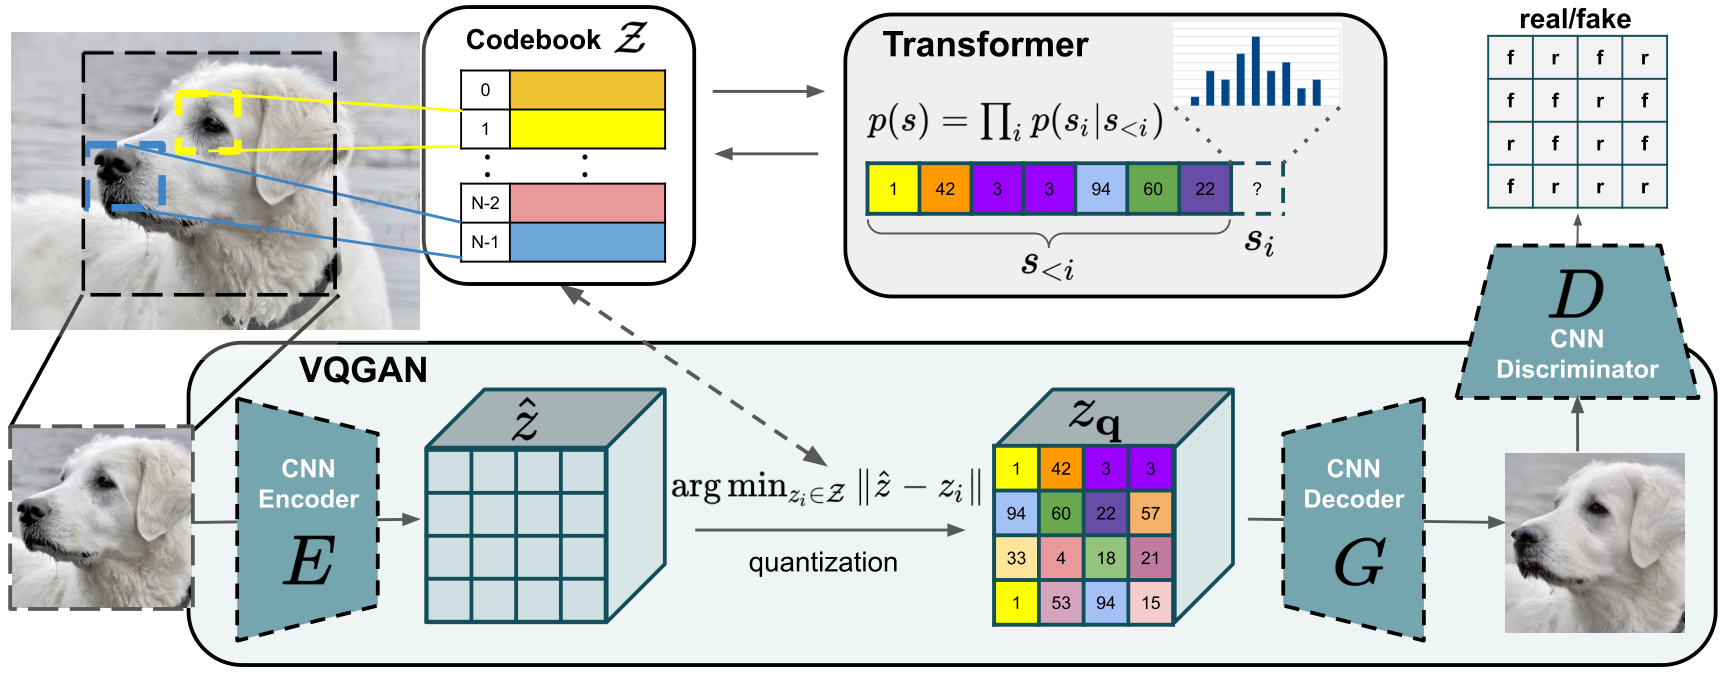
\includegraphics[width=0.8\linewidth]{figs/taming_transformers_1}
	\end{figure}
	\begin{figure}
		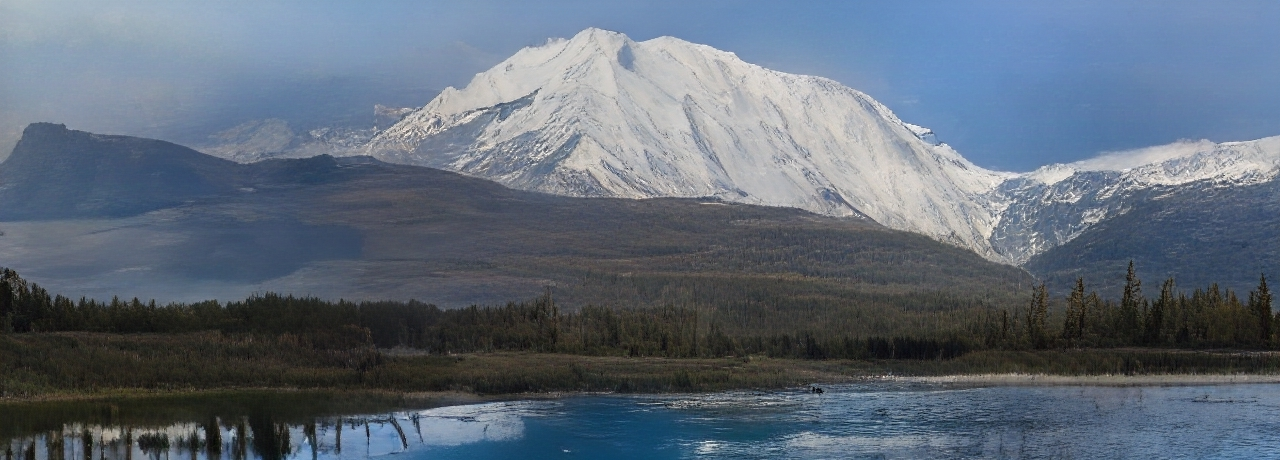
\includegraphics[width=\linewidth]{figs/taming_transformers_2}
	\end{figure}
\myfootnotewithlink{https://arxiv.org/abs/2012.09841}{Esser P., Rombach R., Ommer B. Taming Transformers for High-Resolution Image Synthesis, 2020}
\end{frame}
%=======
\begin{frame}{Problem Statement}
We are given i.i.d. samples $\{\bx_i\}_{i=1}^n \in X$ (e.g. $X = \bbR^m$) from unknown distribution $\pi(\bx)$.

\begin{block}{Goal}
	We would like to learn a distribution $\pi(\bx)$ for 
	\begin{itemize}
	    \item evaluating $\pi(\bx)$ for new samples (how likely to get object $\bx$?);
	    \item sampling from $\pi(\bx)$ (to get new objects $\bx \sim \pi(\bx)$).
	\end{itemize}
\end{block}
\begin{block}{Challenge}
	 Data is complex and high-dimensional. Imagine the dataset of images which lies in the space $X \subset \bbR^{\text{width} \times \text{height}}$.
\end{block}
\end{frame}
%=======
\begin{frame}{Histogram as a generative model}
	
	\begin{minipage}[t]{0.6\columnwidth}
	    Let $x \sim \text{Categorical}$. The histogram is totally defined by
		\[
		    \pi_k = \pi(x = k) = \frac{\sum_{i=1}^k [x_i = k]}{n}.
		\]
		MNIST: 28x28 gray-scaled images \\
		each image is $\bx = (x_1, \dots, x_{784})$, where $x_i \sim \text{Be}(p_i)$. \\
		$2^{28\times28} - 1$ parameters to specify $\pi(\bx)$ 
		\end{minipage}%
		\begin{minipage}[t]{0.4\columnwidth}
	    \begin{figure}[h]
	        \centering
	        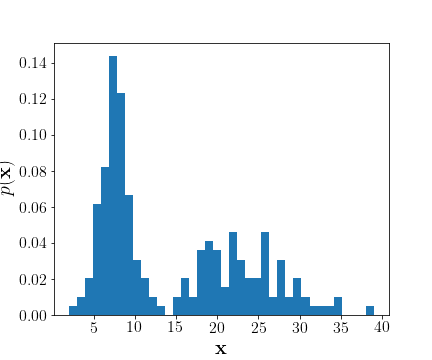
\includegraphics[width=\linewidth]{figs/histogram.png}
	    \end{figure}
	\end{minipage}
	\[
	    \pi(\bx) = \pi(x_1) \cdot \pi(x_2 | x_1) \cdot \dots \cdot \pi(x_m | x_{m-1}, \dots, x_1).
	\]
	\textbf{Question:} How many parameters do we need in these cases?
	\[
	    \pi(\bx) = \pi(x_1) \cdot \pi(x_2)\cdot \dots \cdot \pi(x_m).
	\]
	\[
	    \pi(\bx) = \pi(x_1) \cdot \pi(x_2 | x_1) \cdot \dots \cdot \pi(x_m | x_{m-1}).
	\]
\end{frame}
%=======
\begin{frame}{Maximum likelihood}
    Fix probabilistic model $p(\bx | \btheta)$~-- the set of parameterized distributions . \\
    Instead of searching true $\pi(\bx)$ over all probability distributions, learn function approximation $p(\bx | \btheta) \approx \pi(\bx)$.
    
    \begin{block}{MLE problem}
    \vspace{-0.3cm}
    \[
        \btheta^* = \argmax_{\btheta} p(\bX | \btheta) = \argmax_{\btheta} \prod_{i=1}^n p(\bx_i | \btheta) = \argmax_{\btheta} \sum_{i=1}^n \log p(\bx_i | \btheta).
    \]
    \vspace{-0.1cm}
    \end{block}
    
    The problem is solved with SGD.
    \begin{block}{Requirements}
        \begin{itemize}
            \item efficiently compute $\log p(\bx | \btheta)$;
            \item efficiently compute gradient of $\log p(\bx | \btheta)$.
        \end{itemize}
    \end{block}
\end{frame}
\begin{frame}{Autoregressive model}
    \begin{block}{MLE problem}
    \vspace{-0.5cm}
    \[
        \btheta^* = \argmax_{\btheta} p(\bX | \btheta) = \argmax_{\btheta} \prod_{i=1}^n p(\bx_i | \btheta) = \argmax_{\btheta} \sum_{i=1}^n \log p(\bx_i | \btheta).
    \]
    \vspace{-0.5cm}
    \end{block}
    \begin{block}{Challenge}
    $p(\bx | \btheta)$ could be intractable.
    \end{block}
    \begin{block}{Likelihood as product of conditionals}
    Let $\bx = (x_1, \dots, x_m)$, $\bx_{1:i} = (x_1, \dots, x_i)$. Then 
    \[
        p(\bx | \btheta) = \prod_{i=1}^m p(x_i | \bx_{1:i - 1}, \btheta); \quad 
        \log p(\bx | \btheta) = \sum_{i=1}^m \log p(x_i | \bx_{1:i - 1}, \btheta).
    \]
    \end{block}
	\textbf{Example:} $p(x_1, x_2, x_3) = p(x_2) \cdot p(x_1 | x_2) \cdot p(x_3 | x_1, x_2)$.
\end{frame}
%=======
\begin{frame}{Autoregressive models}
    \[
    \log p(\bx| \btheta) = \sum_{i=1}^m \log p(x_i | \bx_{1:i - 1}, \btheta)
    \]
    \begin{itemize}
	    \item Sampling is sequential:
	    \begin{itemize}
    		\item sample $\hat{x}_0 \sim p(x_1 | \btheta)$;
    		\item sample $\hat{x}_1 \sim p(x_2 | x_1, \btheta)$;
    		\item \dots
    		\item sample $\hat{x}_n \sim p(x_n | \bx_{1:n-1}, \btheta)$;
    		\item new generated object is $\hat{\bx} = (\hat{x}_1, \hat{x}_2, \dots, \hat{x}_n)$.
    	\end{itemize}
        \item Each conditional $p(x_i | \bx_{1:i - 1}, \btheta)$ could be modelled by neural network.
        \item Modelling all conditional distributions separately is infeasible and we would obtain separate models. To extend to high dimensions we could share parameters $\btheta$ across conditionals.

    \end{itemize}
\end{frame}
%=======
\begin{frame}{Autoregressive models}
		For large $i$ the conditional distribution $p(x_i | \bx_{1:i - 1}, \btheta)$ could be infeasible. Moreover, the history $\bx_{1:i-1}$ has non-fixed length.
		\begin{block}{Markov assumption}
			\vspace{-0.5cm}
			\[
				p(x_i | \bx_{1:i - 1}, \btheta) = p(x_i | \bx_{i - d:i - 1}, \btheta), \quad d \text{ is a fixed model parameter}.
			\]
		\end{block}
		\begin{block}{Example}
			\begin{minipage}[t]{0.39\columnwidth}
				{\small
				\begin{itemize}
					\item $d = 2$;
					\item $x_i \in \{0, 255\}$;
					\item $\bh_i = \text{MLP}_{\btheta}(x_{i - 1}, x_{i - 2})$;
					\item $\bp_i = \text{softmax}(\bh_i)$;
					\item $p(x_i | x_{i - 1}, x_{i - 2}, \btheta) = \text{Categorical}(\bp_i)$.
				\end{itemize}
				}
			\end{minipage}%
			\begin{minipage}[t]{0.61\columnwidth}
			    \begin{figure}
			        \centering
			        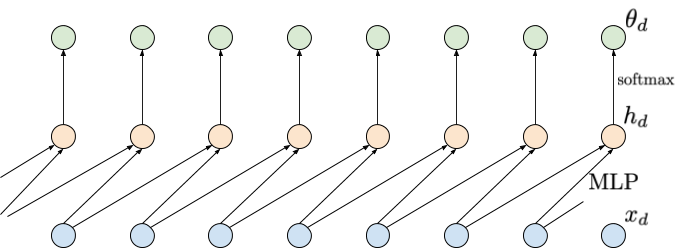
\includegraphics[width=1.0\linewidth]{figs/sequential_MLP}
			    \end{figure}
			\end{minipage}
		\end{block}
	    \myfootnotewithlink{https://jmtomczak.github.io/blog/2/2\_ARM.html}{image credit: https://jmtomczak.github.io/blog/2/2\_ARM.html}
\end{frame}
%=======
\begin{frame}{Autoregressive models}
	\begin{itemize}
		\item Previous model has \textbf{limited} memory $d$. It is insufficient for many modalities (e.g. for images and text). 
		\item Recurrent NN fixes this problem and potentially could learn long-range dependencies:
		\[
			p(x_i | \bx_{1:i - 1}, \btheta) = p(x_i | \bh_i, \btheta), \quad \bh_i = \text{RNN}(\bx_{i - 1}, \bh_{i - 1})
		\]
		 \begin{figure}
	    \centering
	    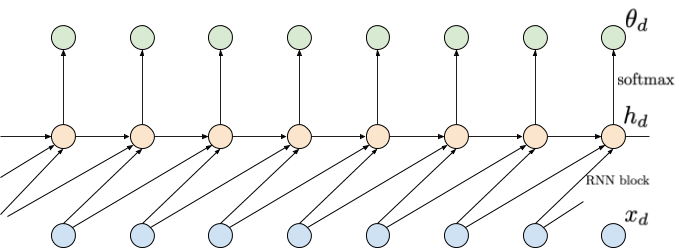
\includegraphics[width=0.7\linewidth]{figs/sequential_RNN}
		 \end{figure}
		\item Sequential computation of all conditionals $p(x_i | \bx_{1:i-1}, \btheta)$, hence, the training is slow.
		\item RNN suffers from vanishing and exploding gradients.
	\end{itemize}
	 \myfootnotewithlink{https://jmtomczak.github.io/blog/2/2\_ARM.html}{image credit: https://jmtomczak.github.io/blog/2/2\_ARM.html}
\end{frame}
%=======
\begin{frame}{Char RNN}
	Model tries to predict the next token (single letter) from previous context.
	\begin{minipage}[t]{0.55\columnwidth}
		\begin{figure}
			\centering
			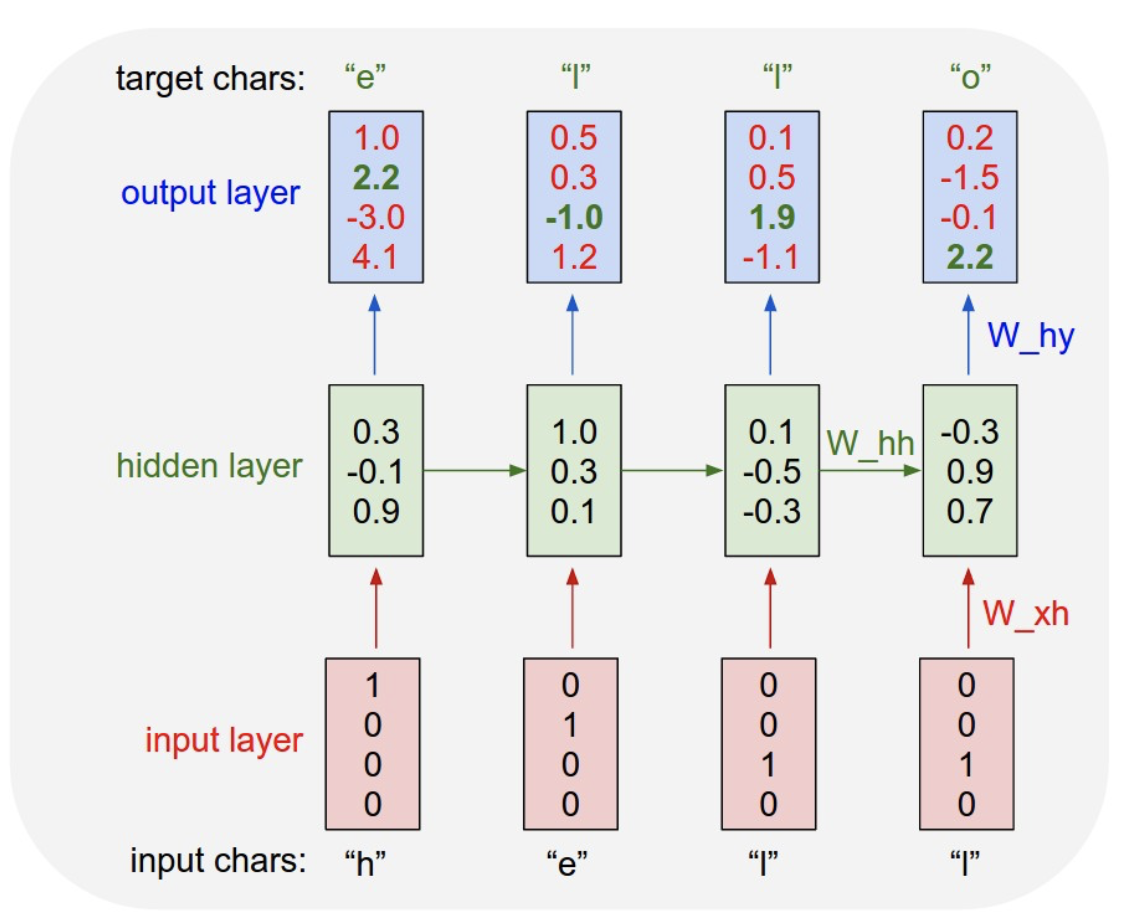
\includegraphics[width=1.0\linewidth]{figs/char_rnn.png}
		\end{figure}
	\end{minipage}%
	\begin{minipage}[t]{0.44\columnwidth}
		\begin{figure}
			\centering
			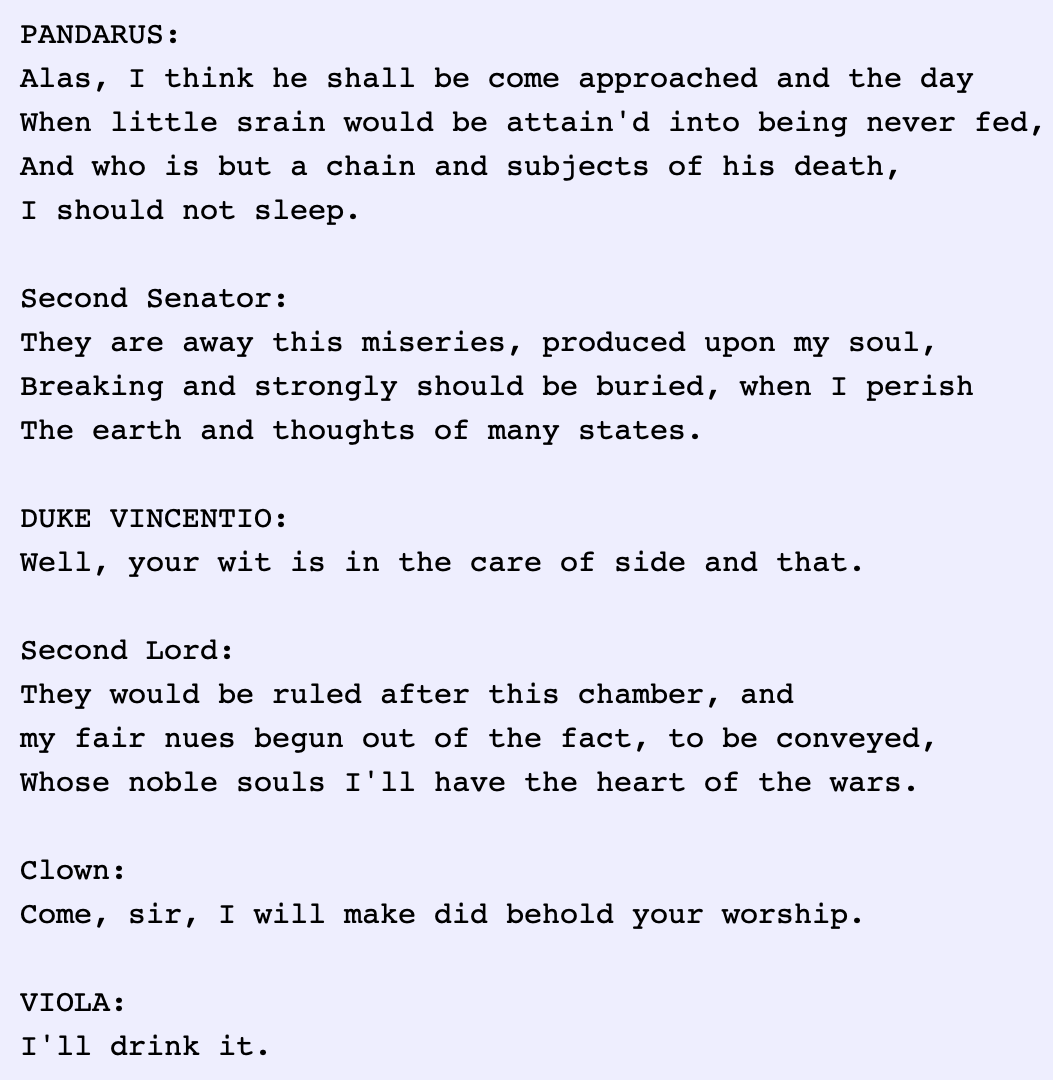
\includegraphics[width=1.0\linewidth]{figs/char_rnn_output.png}
		\end{figure}
	\end{minipage}
\myfootnotewithlink{http://karpathy.github.io/2015/05/21/rnn-effectiveness/}{image credit: http://karpathy.github.io/2015/05/21/rnn-effectiveness}
\end{frame}
%=======
\begin{frame}{Autoregressive models}
		\begin{itemize}
			\item Convolutions could be used for autoregressive models, but they have to be \textbf{causal}. \\
			\item Try to find and understand the difference between Conv A/B.
		    \begin{figure}
		        \centering
		        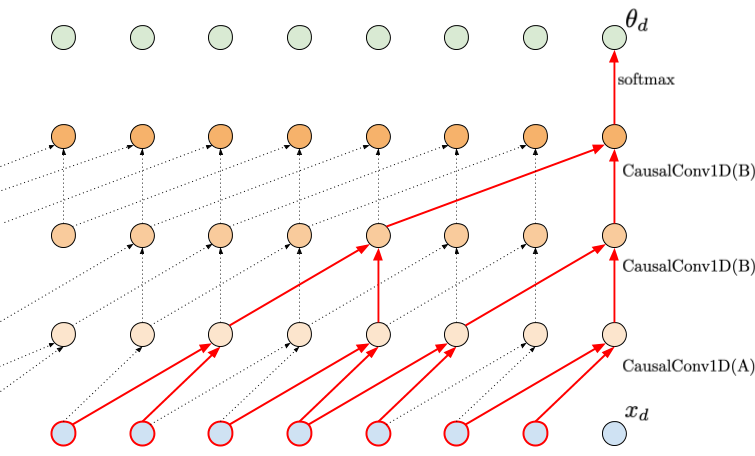
\includegraphics[width=0.7\linewidth]{figs/sequential_CNN}
		    \end{figure}
		    \item Could learn long-range dependecies.
		    \item Do not suffer from gradient issues.
		    \item Easy to estimate probability for given input, but hard generation of new samples (the sequential process).
	   	\end{itemize}
	    \myfootnotewithlink{https://jmtomczak.github.io/blog/2/2\_ARM.html}{image credit: https://jmtomczak.github.io/blog/2/2\_ARM.html}
\end{frame}
%=======
\begin{frame}{MADE}
	\begin{itemize}
		\item Vanila autoencoder is not a generative model. Why?
		\item Let mask the weight matrices to make the model generative: $\bW_M = \bW \cdot \bM$.
		\begin{figure}
		    \centering
		    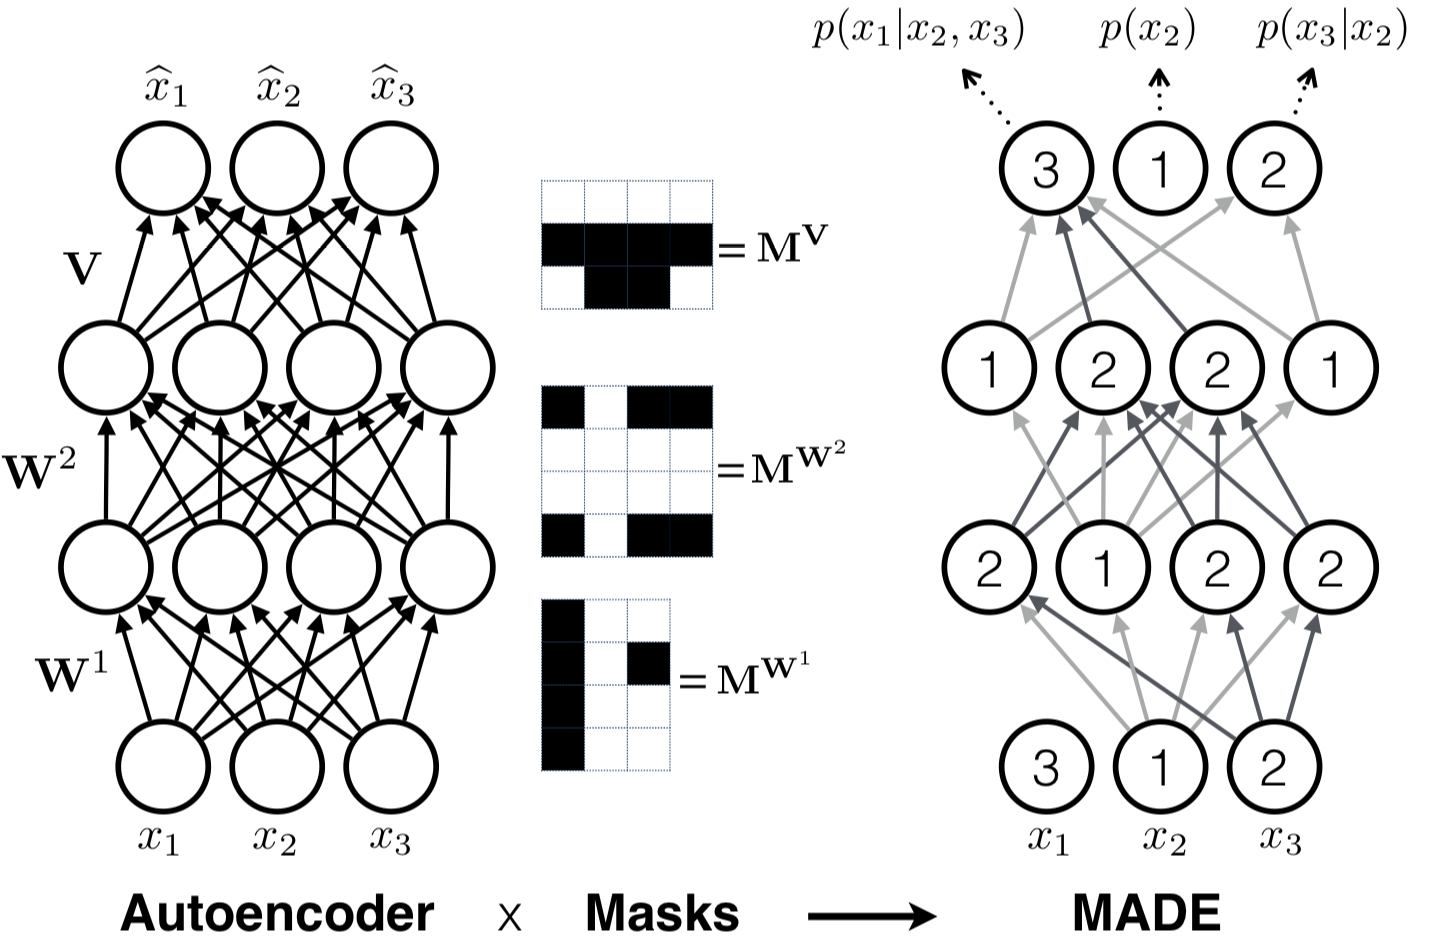
\includegraphics[width=0.7\linewidth]{figs/made}
		\end{figure}
		\item The question is how to create matrices $\bM$ which produce the autoregressive property?
	\end{itemize}
	\myfootnotewithlink{https://arxiv.org/abs/1502.03509}{Germain M. et al. Made: Masked autoencoder for distribution estimation, 2015}
\end{frame}
%=======
\begin{frame}{MADE}
		\begin{minipage}[t]{0.65\columnwidth}
		    \vspace{-0.5cm}
			\begin{block}{Masks generation}
				\begin{itemize}
					\item Define the ordering of input elements from 1 to $n$.
					\item Assign the random number $m$ from 1 to $n - 1$ to each hidden unit. The number gives the
					maximum number of input units to which the unit can be connected.
					\item Connect each hidden unit with number $m$ with the previous layer units which has the number is \textbf{less or equal} than~$m$.
					\item Connect each output unit with number $m$ with the previous layer units which has the number is \textbf{less} than $m$.
				\end{itemize}
			\end{block}
		\end{minipage}%
		\begin{minipage}[t]{0.33\columnwidth}
			\vspace{2cm}
			\begin{figure}
				\centering
				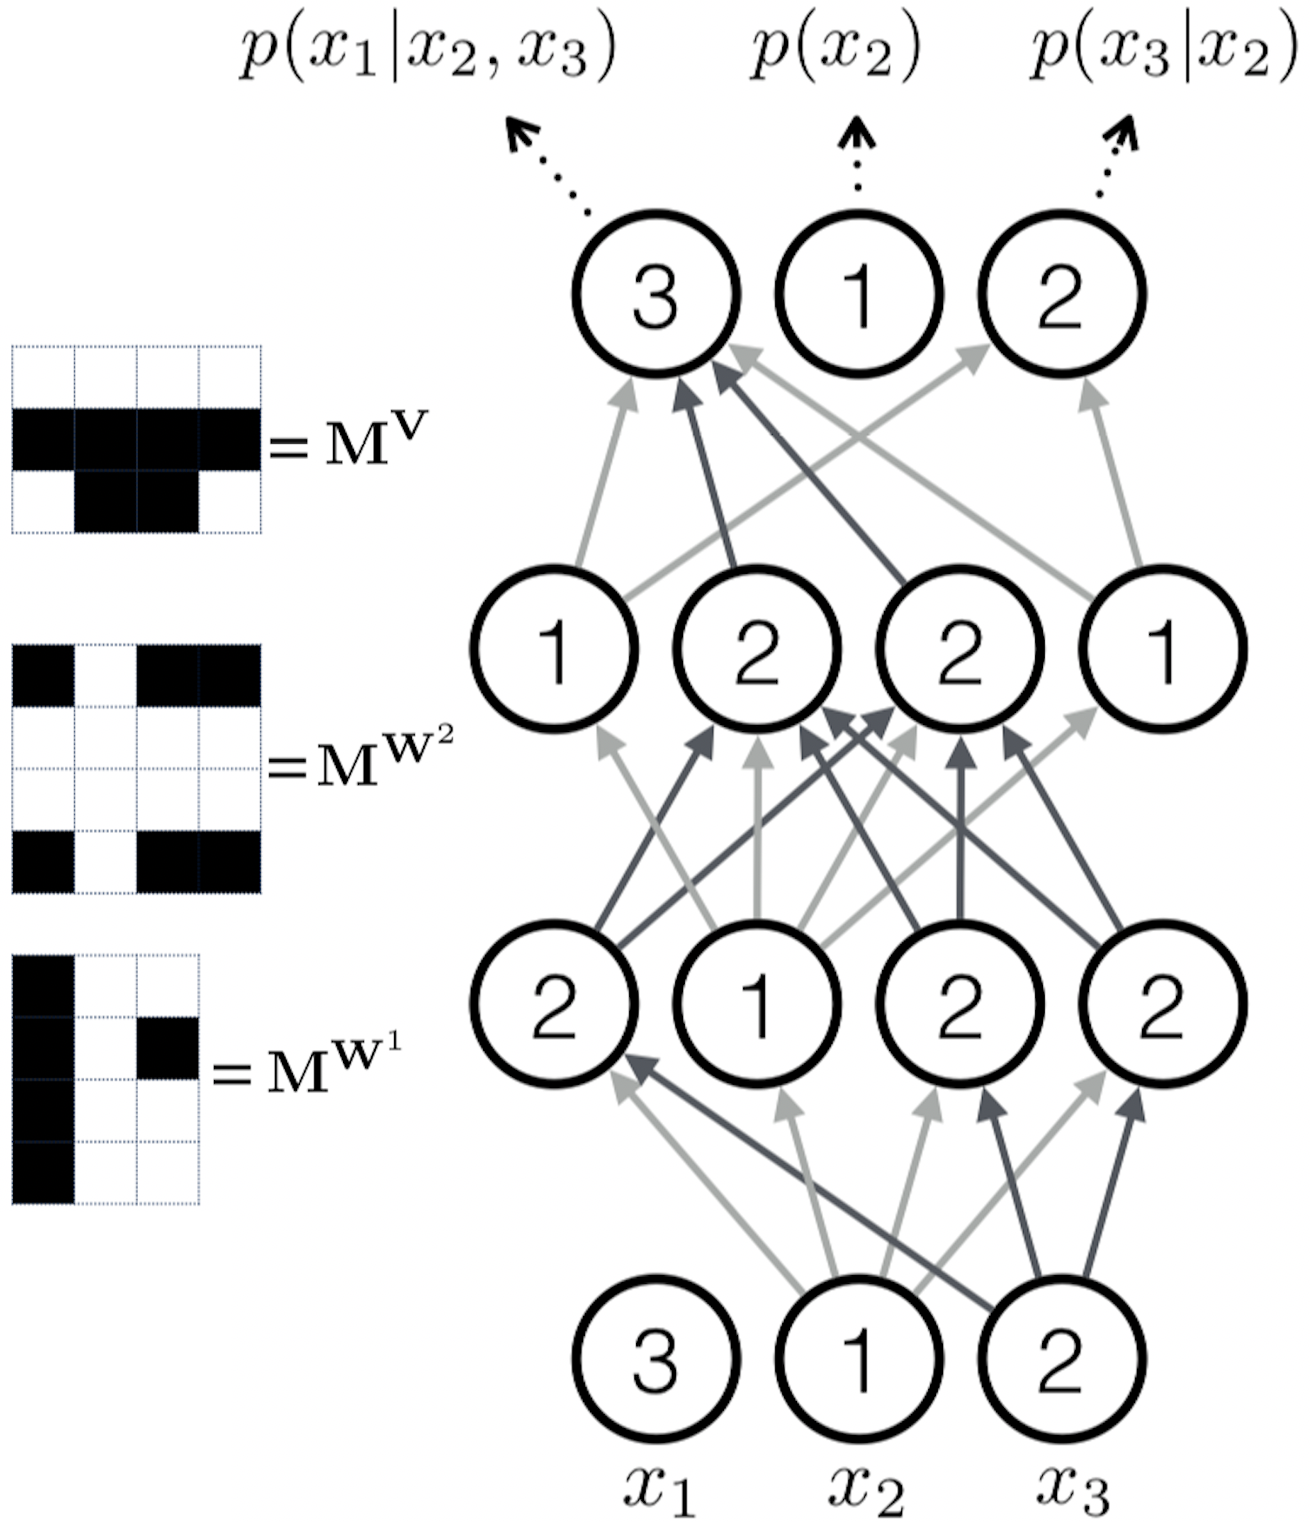
\includegraphics[width=1.0\linewidth]{figs/made2}
			\end{figure}
		\end{minipage}
	\myfootnotewithlink{https://arxiv.org/abs/1502.03509}{Germain M. et al. Made: Masked autoencoder for distribution estimation, 2015}
\end{frame}
%=======
\begin{frame}{WaveNet}
	\begin{block}{Goal}
	Efficient generation of raw audio waveforms with natural sounds.
	\end{block}
	\begin{figure}
	  \centering
	  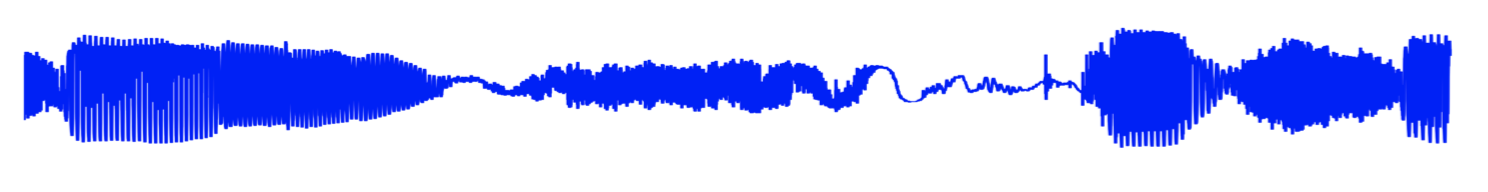
\includegraphics[width=0.9\linewidth]{figs/wavenet_ex.png}
	\end{figure}
	\begin{block}{Solution}
		Autoregressive model
		\vspace{-0.3cm}
		\[
		    p(\bx| \btheta) = \prod_{t=1}^T p(x_t|\bx_{1:t-1}, \btheta).
		\]
		\vspace{-0.3cm}
	\end{block}
	\begin{itemize}
		\item Each conditional $p(x_t|\bx_{1:t-1}, \btheta)$ models the distribution for the timestamp $t$.
		\item The model uses \textbf{causal} dilated convolutions.
	\end{itemize}
	\myfootnotewithlink{https://arxiv.org/abs/1609.03499}{Oord A. et al. Wavenet: A generative model for raw audio, 2016}
\end{frame}
%=======
\begin{frame}{WaveNet (2016)}
	\begin{figure}
	    \centering
	    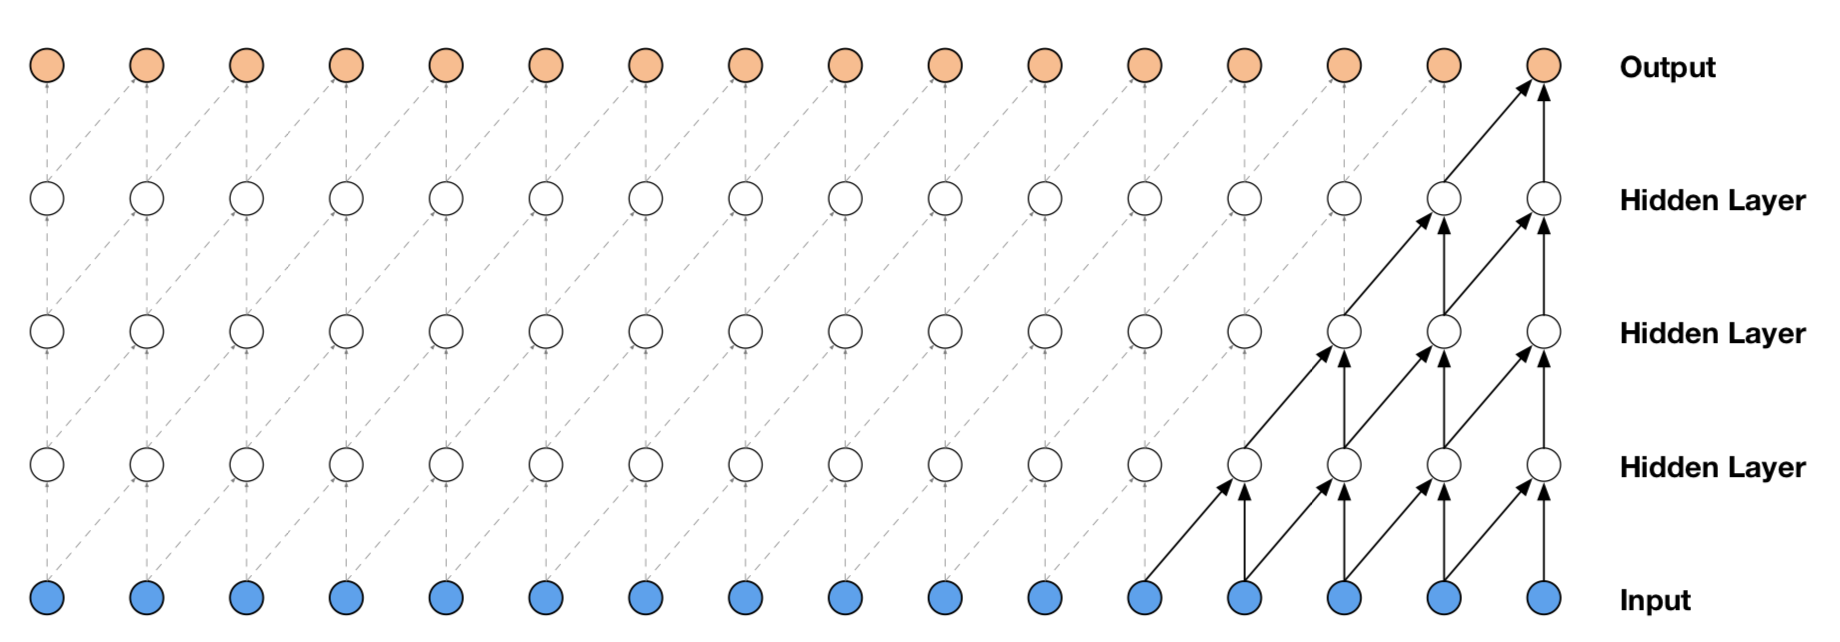
\includegraphics[width=0.9\linewidth]{figs/wavenet1.png}
	\end{figure}
	
	\begin{figure}
	    \centering
	    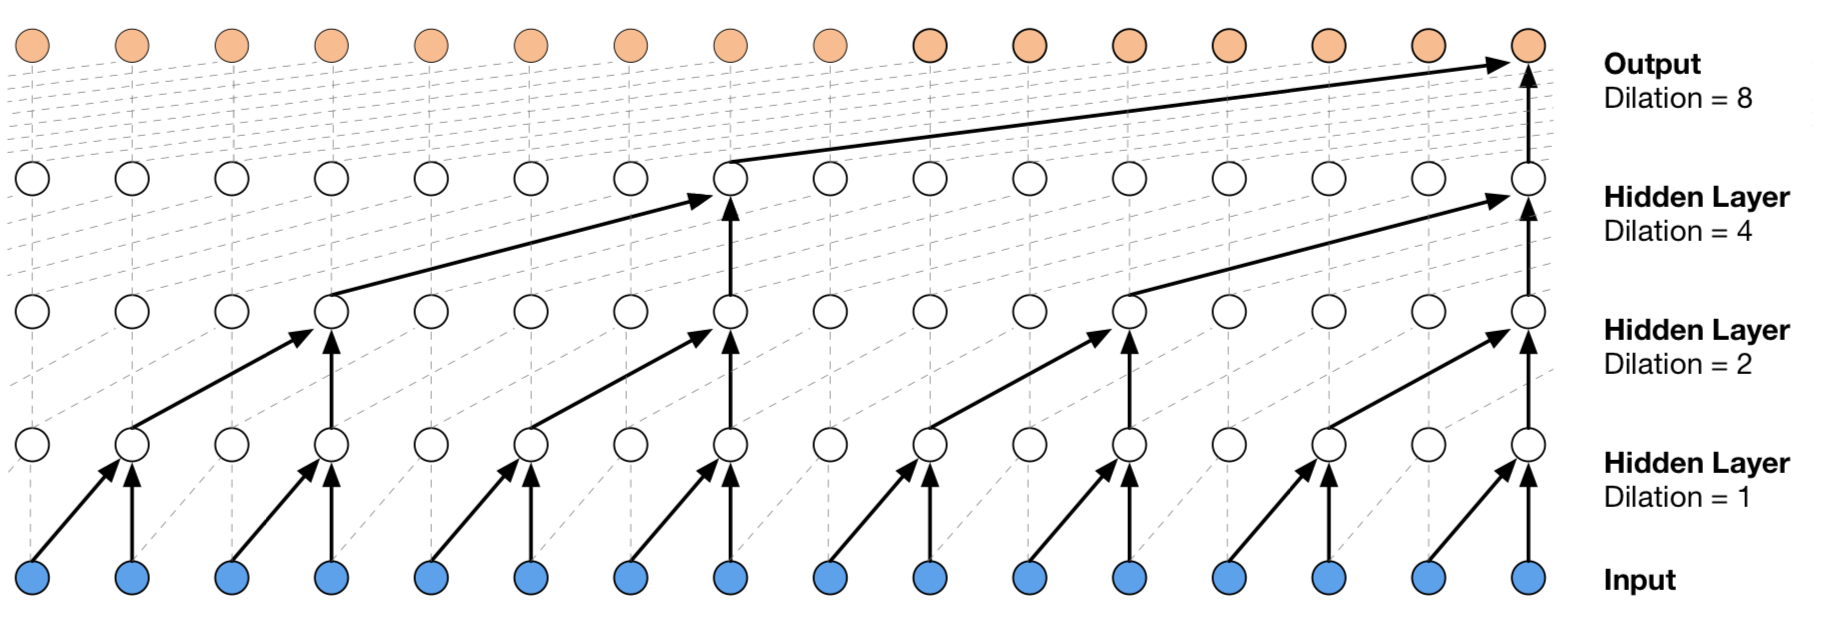
\includegraphics[width=0.9\linewidth]{figs/wavenet2.png}
	\end{figure}
	\myfootnotewithlink{https://arxiv.org/abs/1609.03499}{Oord A. et al. Wavenet: A generative model for raw audio, 2016}
\end{frame}
%=======
\begin{frame}{PixelCNN}
	\begin{block}{Goal}
	Model a distribution of natural images.
	\end{block}
	\begin{block}{Solution}
	Autoregressive model
	\[
	    p(\bx | \btheta) = \prod_{i=1}^{n^2} p(x_i|\bx_{1:i-1}, \btheta).
	\]
	\begin{itemize}
	    \item \textbf{masked} convolutions;
	    \item dependencies over RGB channels.
	\end{itemize}
	\end{block}
	\myfootnotewithlink{https://arxiv.org/abs/1601.06759}{Oord A., Kalchbrenner N., Kavukcuoglu K. Pixel recurrent neural networks, 2016}
\end{frame}
%=======
\begin{frame}{PixelCNN (2016)}
\begin{minipage}[t]{0.5\columnwidth}
	\begin{figure}[h]
		\centering
        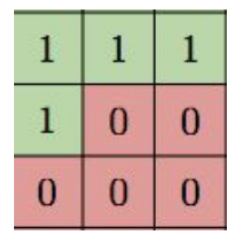
\includegraphics[width=0.35\linewidth]{figs/pixelcnn_0_1.png}
	\end{figure}
	\vspace{-0.1cm}
	\begin{figure}[h]
		\centering
        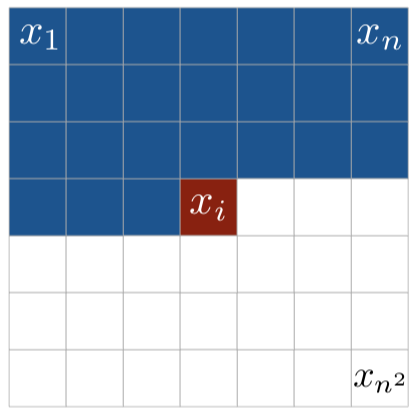
\includegraphics[width=0.7\linewidth]{figs/pixelcnn1.png}
	\end{figure}
	\end{minipage}%
	\begin{minipage}[t]{0.5\columnwidth}
	\begin{figure}[h]
		\centering
        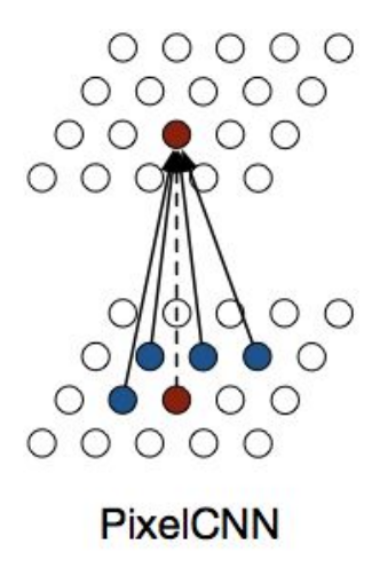
\includegraphics[width=0.5\linewidth]{figs/pixelcnn_0_2.png}
	\end{figure}
	\vspace{-0.4cm}
	\begin{figure}
		\centering
        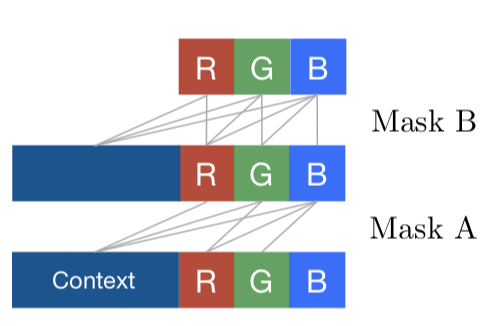
\includegraphics[width=0.65\linewidth]{figs/pixelcnn2.png}
	\end{figure}
\end{minipage}
\myfootnotewithlink{https://arxiv.org/abs/1601.06759}{Oord A., Kalchbrenner N., Kavukcuoglu K. Pixel recurrent neural networks, 2016}
\end{frame}
%=======
\begin{frame}{Summary}
    \begin{itemize}
        \item Sampling from autoregressive models is trivial, but sequential
        \begin{itemize}
            \item sample $x_0 \sim p(x_0)$;
            \item sample $x_1 \sim p(x_1 | x_0)$;
            \item \dots.
        \end{itemize}
        \item Estimating probability:
        \[
            p(\bx) = \prod_{i=1}^m p(x_i | \bx_{1:i - 1}).
        \]
        \item Work on both continuous and discrete data.
        \item There is no natural way to do unsupervised learning.
    \end{itemize}
\end{frame}

\end{document} 